% ============================================================
%  小论文 --- ASR (Advances in Space Research)
%  标题：面向敏捷 SAR 卫星的物理感知多目标调度：权衡收益、NESZ 与几何分辨率
%  中文翻译版本——对应英文版 small-paper-ijae.tex (revision 2026-07-31，已同步)
% ============================================================
\documentclass[preprint,12pt,authoryear]{elsarticle}
% ── 宏包 ──
\usepackage{amsmath,amssymb,amsfonts}
\usepackage{booktabs}
\usepackage{caption}
\captionsetup{justification=centering}
\usepackage{subcaption}
\usepackage{multirow}
\usepackage{enumitem}
\usepackage{float}
\usepackage{hyperref}
\usepackage{xeCJK}
\setCJKmainfont{SimSun}
\graphicspath{{figures/}}
% ── 期刊 ──
\journal{Advances in Space Research}
% ── 元数据 ──
\begin{document}
\begin{frontmatter}
\title{面向敏捷 SAR 卫星的物理感知多目标调度：权衡收益、NESZ 与几何分辨率}
\author{刘书豪}
\ead{liushuhao@hrbeu.edu.cn}
\affiliation{organization={哈尔滨工程大学 智能科学与工程学院},
            addressline={南通大街 145 号},
            city={哈尔滨},
            postcode={150001},
            country={中国}}
% ============================================================
%  摘要
% ============================================================
\begin{abstract}
在敏捷 SAR 调度中，观测时机不仅决定了可行性，还通过雷达特有的几何和辐射效应影响成像质量。
本文通过将两个物理质量维度——噪声等效后向散射系数（NESZ，辐射度量）和几何分辨率——作为
非支配排序遗传算法 III（NSGA-III）框架内的分解优化目标，刻画了单次过境、单星条带模式 SAR 多目标质量优化的经验饱和态势，
区别于先前 SAR 调度中使用的标量可见性复合指标。
此处 $f_1^*$ 表示归一化覆盖收益，$f_2$ 表示平均几何图像质量，$f_3$ 表示平均 NESZ 辐射质量；
三者均以越大越优。
在 20 到 500 目标密度的实验中显示了一个尺度依赖的饱和：在最稀疏密度（$N = 20$）下，
多目标优化以 $13\%$ 的覆盖率代价换取 $f_2$ 的 $+4.5\%$ 几何质量提升（MOEA-2），
而加入 NESZ 目标 $f_3$ 后，仅以 $2\%$ 覆盖率代价即相对 G-BL 获得 $+58\%$ 的辐射质量增益（MOEA-3）；
而在运营密度（$N \geq 300$）下，以贪心基线（G-BL）为种子的多目标进化算法（MOEA）公式化趋近贪心覆盖锚点，边际质量增益低于 $2\%$。
该覆盖收敛以贪心基线热启动为先决条件，随机初始化的 $f_1^*$ 差距为 $0.24$--$0.68$，并在中高目标密度处达到峰值。
独立地，消融实验显示去除物理目标几乎不改变密集场景结果。
第三个目标因此是密度依赖的而非冗余的：MOEA-3 在稀疏密度下与 MOEA-2 明显不同
（$f_3$ 相对 MOEA-2 提升 $+84\%$），而在运营密度下收敛，
反映了低斜视区域的几何耦合而非目标间的数学恒等关系。本文并非识别出某个更优的求解器，
而是在本文测试的单星、单过境、条带模式、以 G-BL 热启动的 NSGA-III 条件下，建立了物理感知多目标调度的经验饱和边界。
\end{abstract}
\begin{keyword}
敏捷 SAR \sep 卫星调度 \sep 多目标优化 \sep NSGA-III \sep 噪声等效后向散射系数（NESZ）\sep 几何分辨率
\end{keyword}
\end{frontmatter}
% ============================================================
%  1. 引言
% ============================================================
\section{引言}
配备合成孔径雷达（SAR）的敏捷地球观测卫星在从灾害响应到海上监视等
时间关键型任务中日益重要。
其敏捷性——天线波束偏离星下点轨迹的能力——使单颗卫星能够比固定指向平台
在每个轨道上成像更多目标 \citep{Curlander1991}。
然而，这种灵活性将调度从简单的可行性检查转化为一个组合优化问题：
对于 $N$ 个各具有有限可见窗口的目标，调度器必须选择子集并分配满足姿态转换约束的观测时间，
同时最大化某种任务价值度量。
在传统卫星调度中，观测质量通常被表示为每个预计算机会的固定属性，
而非随所选获取时间变化的量。因此，调度问题简化为在时间可行性约束下
最大化观测目标的数量或优先级加权和。
这一假设支撑了大多数现有卫星调度工作，
从混合整数规划公式化到深度强化学习方法 \citep{Chen2025NeuralPriority}。

SAR 成像本质上偏离了这一假设。图像质量取决于获取时刻的雷达几何：
地面距离分辨率随入射角退化（$\rho_{\text{rg}} \propto 1/\sin\theta$），
方位分辨率随斜视角展宽（$\rho_{\text{az}} \propto 1/\cos\psi_{\text{sq}}$），
辐射灵敏度（噪声等效后向散射系数 NESZ）随斜距按 $R^3$ 恶化 \citep{Cumming2005}。
当调度器可以选择在可见窗口内的观测时刻时——这是敏捷卫星的定义特征——
它同时选择了每个目标的成像质量。
尽管调度与成像物理之间存在紧密耦合，除少数例外 \citep{Wei2025MONP,Kramer2025SARVis}，
现有敏捷 SAR 调度方法要么将 SAR 简化为仅覆盖目标，要么对覆盖率最大化求解器产生的调度
应用事后质量检查。
很少有方法将物理质量维度作为 SAR 领域的首要优化目标。

该问题通过时间依赖利润的定向问题归约 \citep{Peng2019Orienteering} 被证明为 NP-hard，
排除了除最小实例外所有情况下的多项式时间精确算法。
SAR 文献已建立了 NESZ 和几何分辨率作为观测几何函数的成熟模型 \citep{Curlander1991,Cumming2005}，
多目标优化文献提供了如 NSGA-III \citep{Deb2014} 等成熟框架用于同时处理三个或更多目标。
然而，这三类要素的直接整合——SAR 物理建模、多目标进化算法（MOEA）和卫星调度——
仍有限。因此，我们将 SAR 调度公式化为在 MOEA 框架内具有独立、物理导出的几何和辐射质量目标。

我们公式化了一个三目标敏捷 SAR 调度问题，其中调度器同时优化：
(1) 总覆盖收益，(2) 平均几何图像质量（地面距离和方位分辨率），
以及 (3) 平均 NESZ 辐射质量。
我们比较了五种涵盖方法论谱系的求解器：两种贪心启发式（一种仅收益基线和一种最小化斜视变体），
一种具有贪心热启动的单目标遗传算法，以及两种具有两个和三个目标的 NSGA-III 变体。
这些求解器在跨越四个密度类别的 200 个系统变化场景上进行了评估
（$N = 20$ 到 $N = 500$）。
我们的结果揭示了一个尺度依赖的饱和而非统一的求解器优势。
在稀疏场景中，多目标优化可以提取适度的几何质量增益
——但代价是覆盖率的显著下降，仅选择简单贪心调度器捕获目标的一小部分。
在密集场景中，多目标优势减小到可忽略的水平：
贪心方法接近帕累托最优覆盖，最小化斜视启发式提供了有竞争力的辐射质量。
第~\ref{sec:summary} 节提供了这些发现的详细综合。
本文的具体贡献包括：
\begin{enumerate}[nosep]
    \item 发现并分析刻画了单次过境、单星条带设置中多目标 SAR 质量优化的
    经验饱和态势：该态势源于求解器收敛到低斜视区域，
    抑制了 $\theta$ 轴上几何质量与辐射质量之间的冲突
    （\S~\ref{sec:pareto-coupling}），
    而非目标间的物理恒等关系，并使得三目标公式化在运营密度下变得冗余。
    受控消融研究（四种目标函数变体，每种 200 场景）确认了
    在高目标密度下求解器结果对物理目标的选择不变，
    初始化对照（\S~\ref{sec:robustness-calibration}）则确认
    覆盖收敛以贪心基线（G-BL）热启动为先决条件；
    \item 将 SAR 图像质量分解为封闭形式的 NESZ
    （$\propto R^3$）和几何质量指标（$\sin\theta\cos\psi_{\text{sq}}$）
    目标，置于 NSGA-III 框架内——区别于
    \citet{Kramer2025SARVis} 的标量可见性复合指标和
    \citet{Wei2025MONP} 的通用图像质量复合指标——
    使用每任务平均质量度量，将质量与调度任务数量解耦。
    该公式化使得在四种尺度类别（200 场景）上，跨越贪心启发式、
    单目标 GA 和 NSGA-III 变体的五种求解器的质量-覆盖权衡的系统刻画成为可能。
\end{enumerate}
% ============================================================
%  2. 相关工作
% ============================================================
\section{相关工作}
我们回顾本文所衔接的三个研究方向：卫星调度（2.1）、SAR 物理质量建模（2.2）
和多目标进化优化（2.3）。
\subsection{卫星调度}
卫星调度在地球观测领域得到了广泛研究。\citet{Ferrari2025} 的综述编录了超过 200 篇
涵盖精确方法、启发式、元启发式和基于学习方法的文献。
基于混合整数线性规划（MILP）的精确公式化在小规模实例上可以达到最优，
但无法扩展到运营规模的问题，这推动了包括遗传算法、模拟退火和禁忌搜索在内的
广泛启发式和元启发式替代方案 \citep{Wang2019MILP,Chen2019MILPMulti}。
\citet{Lemaitre2002MultiSat} 和 \citet{Bianchessi2007} 对敏捷卫星调度的
最早正式处理建立了时间依赖观测间转换时间的基本问题结构。
近期工作进一步将这些方法推广到敏捷卫星，利用在每个可见窗口内选择观测开始时间的自由度
在单次轨道中打包更多观测 \citep{Peng2019Orienteering,Chen2024LearnConstruct}。
另一条研究路线追求了基于学习和混合方法的卫星调度。
\citet{Liu2024TwoStageDRL} 和 \citet{Zhou2025TwoPhase} 将深度强化学习应用于
敏捷光学卫星调度，而 \citet{Jacquet2024GNN} 则将图神经网络与蒙特卡洛树搜索
结合用于同一领域。
\citet{Wang2026Lagrangian} 提出了一种基于拉格朗日松弛的启发式方法用于多星任务规划。
\citet{Caleiras2026SuperAgile} 将超敏捷卫星调度建模为约束规划问题，
捕捉了超敏捷平台特征性的时间依赖转换约束。
\citet{Herrmann2023} 将强化学习应用于星载 AEOS 调度，最大化目标收集奖励而不将成像质量作为目标。
\citet{Wu2026WhaleHighDensity} 使用改进鲸鱼优化算法处理高目标密度 AEOS 调度，
报告了与我们分析中的密度驱动约束收紧相呼应的收敛挑战。
尽管方法论多样，大多数先前工作都将质量视为在观测窗口生成时确定的固定属性。
相比之下，SAR 成像质量随采集几何连续变化，且可在调度窗口内直接优化。
\citet{Chang2022Gaofen} 提出了一种用于 SAR 卫星调度的早期 MOEA，在高分 12 号 X 波段 SAR 平台上
使用两种自适应 NSGA-II 变体；其双目标公式化（收益 + 能耗）是与我们最接近的先前工作，
但它省略了成像质量维度。
\citet{Wei2025MONP} 引入了一种神经策略引导的 MOEA，将复合图像质量分数作为优化目标。
\citet{Kramer2025SARVis} 使用混合元启发式方法调度 SAR 星座观测，采用加权可见性-性能复合指标，
在调度器中嵌入 SAR 质量代理，而 \citet{Yao2024Bilevel} 则为多星调度开发了一种
双层进化算法，将任务分配与详细观测规划分离。
所有这些先前工作的共同局限是：SAR 物理质量度量——噪声等效后向散射系数（NESZ）、
方位分辨率、地面距离分辨率——要么缺失，要么被粗略的代理指标近似（例如，惩罚极端离轴角）。
据我们所知，尚无现有 SAR 调度方法将连续的、物理推导的质量函数作为分解的优化目标本身；
最接近的方法嵌入的是聚合质量代理，而非分离的几何与辐射目标。
\subsection{SAR 物理质量建模}
SAR 遥感文献提供了将观测几何与图像质量关联的完善分析模型。
\citet{Curlander1991}、\citet{Cumming2005} 和 \citet{Moreira2025} 给出了 SAR 物理的
全面处理，包括与调度相关的两个质量维度：几何分辨率和辐射灵敏度。
几何分辨率分解为地面距离分辨率 $\rho_{\text{rg}} = c / (2B \sin\theta)$，
其中 $c$ 为光速，$B$ 为雷达带宽，$\theta$ 为入射角，以及方位分辨率
$\rho_{\text{az}} = D / (2 \cos\psi_{\text{sq}})$，其中 $D$ 为天线长度，
$\psi_{\text{sq}}$ 为斜视角。这给出了无加权理论极限；在运营 SAR 中，
Taylor 或 Hamming 幅度加权使 $\rho_{\text{az}}$ 展宽 10--20\% \citep{Curlander1991}。
由于该加权是平台常数，无加权形式保留了观测几何的相对排序以用于优化目的。
两个分量对偏离零多普勒几何（$\psi_{\text{sq}} = 0$，$\theta$ 最小）的响应相反：
$\rho_{\text{az}}$ 随 $|\psi_{\text{sq}}|$ 增大而退化，而 $\rho_{\text{rg}}$
在最近点的最小入射角处最粗、随 $\theta$ 升高反而改善——这正是
\S~\ref{sec:objective-functions} 形式化的 $\theta$ 轴权衡的起源。
辐射灵敏度，由噪声等效后向散射系数（NESZ）度量，随斜距的立方恶化：
$\text{NESZ} \propto R^3 \propto 1/(\cos^3\theta \cdot \cos^3\psi_{\text{sq}})$
（条带 SAR 经方位压缩增益后）\citep{Curlander1991}。
比例关系 $\text{NESZ} \propto R^3$ 捕捉了主要的几何依赖关系；噪声系数、发射功率和处理增益项
被省略，因为它们是平台常数，不影响调度器优化的观测几何相对排序。
这种对斜距的立方依赖意味着即使适度偏离最佳观测几何，也使精细观测时机对辐射性能至关重要。
\citet{Moreira2025} 调查了星载 SAR 技术的演进，并强调成像质量与采集几何内在相关。
这些质量模型在 SAR 系统设计中常规用于指定性能包络（例如，条带上的最大 NESZ）。
然而，它们在调度中的使用仍限于固定观测计划的事后验证 \citep{KramerMiller2024}
或在观测窗口层面的二元可行性过滤 \citep{QualityScreening2026}（arXiv 预印本）。
调度文献和 SAR 质量建模文献一直在并行发展：调度器将质量视为约束，
而 SAR 工程师在调度确定后计算质量。我们的工作通过将连续质量函数直接嵌入优化目标空间，
连接了这两个领域。
\subsection{多目标进化优化}
多目标进化算法（MOEA）已发展为处理两个或更多竞争性目标的标准工具包。
NSGA-III 算法 \citep{Deb2014} 通过基于参考点的多样性保持机制，
将著名的 NSGA-II 框架扩展到多目标问题（$M \geq 3$），
取代了在更高维度上退化的拥挤距离算子。NSGA-III 已应用于航空航天轨迹优化、
星座设计和任务规划问题，其中燃料消耗、覆盖率和重访时间等目标必须同时平衡。
在卫星调度中，MOEA 主要应用于光学领域，目标包括总收益、任务完成时间、
资源利用率和负载均衡。
超体积（HV）指标是比较帕累托前沿近似最广泛使用的质量度量，
但其对前沿基数的敏感性在比较单目标和多目标求解器时产生了可解释性挑战——
我们在 \S~\ref{sec:pareto-coupling} 中处理了这一方法论问题。
据我们所知，MOEA 尚未被应用于具有物理质量目标的 SAR 调度。
最接近的工作使用单目标优化加事后质量评估，这无法揭示覆盖率和成像质量之间
权衡结构的全貌。我们的 NSGA-III 公式化通过将覆盖收益、几何质量和辐射质量
置于统一的多目标框架中，使这些权衡变得明确，产生任务规划者可以检查的帕累托前沿，
以做出明智的质量-覆盖决策。
% ============================================================
%  3. 问题形式化
% ============================================================
\section{问题形式化}
% ── 3.1 系统模型 ──
\subsection{系统模型}\label{sec:system-model}
我们考虑一个在圆形轨道高度 $H$ 上运行的敏捷 SAR 卫星，采用条带模式。
我们选择条带模式作为基线 SAR 模式，因为它提供最宽的连续测绘带且质量均匀，
其质量-几何关系可通过封闭形式的 NESZ 和分辨率表达式进行分析处理 \citep{Curlander1991}。
ScanSAR 和 TOPS 模式的扩展在 \S~\ref{sec:limitations} 中讨论。
问题实例 $\mathcal{I} = (\mathcal{T}, \mathcal{P}, \mathcal{O})$ 由
一组 $N$ 个地面目标 $\mathcal{T}$、一个卫星平台 $\mathcal{P}$ 和一个 SAR 成像模型 $\mathcal{O}$ 组成。
\paragraph{任务集.}
每个任务 $i \in \{1,\ldots,N\}$ 由其地理坐标 $\mathbf{r}_i = (\phi_i, \lambda_i)$、
优先级权重 $p_i \in \mathbb{R}^+$、最小所需地面分辨率 $\rho_i^{\text{req}}$、
可见窗口 $\mathcal{W}_i = [a_i, b_i]$（在此期间卫星可以观测目标）
以及固定观测持续时间 $d_i$ 指定。
\paragraph{卫星平台.}
卫星的特征参数包括最大旋转速率 $\omega_{\max}$（对三轴姿态机动的保守单轴界限）、
每次机动后的稳定时间 $\tau_{\text{settle}}$、每轨道能量预算 $E_{\max}$ 和存储预算 $M_{\max}$，
以及每次观测的能量消耗 $e_i$ 和存储消耗 $m_i$。
\paragraph{SAR 可观测量.}
给定观测时间 $t_i$，卫星到目标的视线（LOS）向量 $\mathbf{l}(t_i)$
在本地垂直本地水平（LVLH）坐标系中由卫星轨道状态完全确定。
从 $\mathbf{l}(t_i)$ 我们确定性地推导出四个几何量：
斜距 $R = |\mathbf{l}|$、离轴角 $\xi = \arctan2(\sqrt{l_x^2+l_y^2},\, l_z)$、
入射角 $\theta$（通过地球曲率校正映射 $\theta = \arcsin\big(\frac{R_e+H}{R_e}\sin\xi\big)$，
其中 $R_e$ 为地球平均半径），以及
斜视角 $\psi_{\text{sq}} = \arcsin(|l_x| / R)$（LVLH $x$ 轴沿轨方向，$z$ 轴指向天底）。
斜视角作为 LOS 向量偏离零多普勒平面的角度偏差的定义遵循 Curlander（1991）
第 9 章 SAR 多普勒特性，其中方位多普勒中心与 $\sin\psi_{\text{sq}}$ 成正比。
一个关键性质是 \emph{所有} 与质量相关的几何量都是单一决策变量 $t_i$ 的确定性函数。
\paragraph{决策变量.}
一个调度方案由任务选择向量 $\mathbf{x} \in \{0,1\}^N$、
有序序列 $S = (s_1,\ldots,s_m)$（$m$ 个选定任务）以及
观测开始时间向量 $\mathbf{t} = (t_{s_1},\ldots,t_{s_m})$ 组成。
所有几何参数（$\theta_i$, $\psi_{\text{sq},i}$, $R_i$）均
从 $t_i$ \emph{推导} 而来，而非独立的决策变量。
% ── 3.2 目标函数 ──
\subsection{目标函数}\label{sec:objective-functions}
我们公式化了一个三目标优化问题，捕捉调度吞吐量与 SAR 特定成像质量之间的张力。
所有质量目标采用选定任务的 \emph{均值}，使其独立于调度任务数量 $m = |\mathcal{S}|$，
从而产生真正的"数量 vs. 质量"帕累托权衡。
\paragraph{目标 1：覆盖收益.}
归一化覆盖收益（式~\ref{eq:f1}）相对于贪心基线定义：
\begin{equation}
f_1^* = \frac{1}{f_1^{\text{G-BL}}} \sum_{i \in \mathcal{S}} p_i
\label{eq:f1}
\end{equation}
其中 $f_1^{\text{G-BL}}$ 是仅收益贪心调度器（G-BL, \S~\ref{sec:gbl}）
在同一场景上实现的收益。
\paragraph{目标 2：几何图像质量.}
SAR 图像的地面像素面积是地面距离分辨率 $\rho_{\text{rg}} = c / (2B \sin\theta)$
与方位分辨率 $\rho_{\text{az}} = D / (2 \cos\psi_{\text{sq}})$ 的乘积。
我们定义无量纲几何质量指标：
\begin{equation}
f_2 = \frac{1}{|\mathcal{S}|} \sum_{i \in \mathcal{S}} \sin\theta_i \cdot \cos\psi_{\text{sq},i}
\label{eq:f2}
\end{equation}
$f_2$ 越高表示地面像素面积越小（几何分辨率越好）。
当 $\mathcal{S} = \emptyset$ 时，$f_2 = 0$。
\paragraph{目标 3：NESZ 辐射质量.}
噪声等效后向散射系数（NESZ）衡量最小可检测后向散射。
对于条带 SAR，NESZ 随斜距的立方恶化：
$\text{NESZ} \propto R^3 \propto 1/(\cos^3\theta \cdot \cos^3\psi_{\text{sq}})$，
经方位压缩增益后 \citep{Curlander1991}。
我们定义辐射质量指标：
\begin{equation}
f_3 = \frac{1}{|\mathcal{S}|} \sum_{i \in \mathcal{S}} \cos^3\theta_i \cdot \cos^3\psi_{\text{sq},i}
\label{eq:f3}
\end{equation}
$f_3$ 越高表示 NESZ 越低（辐射灵敏度越好）。
当 $\mathcal{S} = \emptyset$ 时，$f_3 = 0$。
$f_2$ 和 $f_3$ 均通过构造有界于 $[0,1]$：
$\sin\theta_i$、$\cos\psi_{\text{sq},i}$ 和 $\cos\theta_i$ 均落在本研究所用姿态包络的 $[0,1]$ 内。
\paragraph{物理权衡.}
两个质量目标按物理机制划分 SAR 成像性能：$f_2$ 捕捉空间分辨率（几何），
$f_3$ 捕捉信噪比（辐射）。
它们的最优点并不重合——$f_3$ 在零多普勒点（$\theta$ 最小，$\psi_{\text{sq}} = 0$）达到峰值，
而 $f_2$ 受益于适度较高的 $\theta$，因为 $\sin\theta$ 随入射角增大而增大。
这产生了真正的权衡：追求最干净的 NESZ（零多普勒观测）迫使接受拉伸的地面距离像素；
追求最佳地面像素面积需要偏离零多普勒点并接受升高的辐射噪声。
关键地，斜视角 $\psi_{\text{sq}}$ 同时出现在 $f_2$ 和 $f_3$ 中
（式~\ref{eq:f2}--\ref{eq:f3}）：减小 $\psi_{\text{sq}}$ 通过 $\cos\psi_{\text{sq}}$
因子同时改善两个分辨率分量。实际上，零斜视点与最接近目标的时刻重合，
该时刻斜距最短，且对于球面地球近似使入射角 $\theta$ 最小，从而降低 $\sin\theta$；因此减小 $\psi_{\text{sq}}$
通过两角之间的几何（而非代数）耦合降低 $f_2$，形成双轴 $[\theta, \psi_{\text{sq}}]$
权衡结构，一旦求解器收敛到低斜视区域即限制多目标增益
（式~\ref{eq:rnull} 在 \S~\ref{sec:pareto-coupling} 中及其轴分解，
用于精确定义性和调度器诱导分量的划分）。

由于 $\theta$ 和 $\psi_{\text{sq}}$ 均源自同一 LOS 向量
（\S~\ref{sec:system-model}），每任务的 $f_2$ 和 $f_3$ 贡献共享几何结构。
该耦合的定量刻画——包括定义性零相关性及其与经验求解器结果的比较——
在 \S~\ref{sec:pareto-coupling} 中呈现。
% ── 3.3 约束条件 ──
\subsection{约束条件}
观测窗口成员资格被视为每个起始时间变量的定义域，而非单独的编号约束：
\begin{equation}
t_i \in [a_i, b_i - d_i] \quad \forall i \in \mathcal{S}.
\label{eq:observation-domain}
\end{equation}
其余四个约束将任务选择、获取几何、时间可行性和资源使用耦合在一起。
入射角与斜视角约束（C1）在可见窗口生成期间强制执行；C2--C4 由每个求解器内联检查。

\paragraph{C1：入射角与斜视角约束.}
每个选中的获取必须满足平台的入射角范围 $\theta^{\min} \leq |\theta_i| \leq \theta^{\max}$
和斜视角限制 $|\psi_{\text{sq},i}| \leq \psi_{\text{sq}}^{\max}$，
其中 $\psi_{\text{sq}}^{\max}$ 是卫星的最大可实现斜视角（通常 $45^\circ$）。
两者都是在调度前应用的观测几何限制。

\paragraph{C2：姿态机动与非重叠.}
在连续观测之间，卫星必须旋转经过其 LOS 向量的角度间隔。
设 $\mathbf{l}_k$ 和 $\mathbf{l}_{k+1}$ 分别为 $t_{s_k}$ 和 $t_{s_{k+1}}$ 时刻的 LVLH 坐标系 LOS 向量。
角度间隔 $\Delta\eta_k = \arccos(\mathbf{l}_k\cdot\mathbf{l}_{k+1}/(|\mathbf{l}_k||\mathbf{l}_{k+1}|))$
必须在可用的观测间时间内完成：
\begin{equation}
t_{s_{k+1}} \geq t_{s_k} + d_{s_k} + \frac{\Delta\eta_k}{\omega_{\max}} + \tau_{\text{settle}} \quad \forall k \in \{1,\ldots,m-1\}.
\label{eq:c2}
\end{equation}
此不等式也强制执行非重叠的任务执行区间。它是我们公式化中的核心耦合：改变 $t_{s_k}$ 会移动
$\mathbf{l}_k$，同时影响成像质量（通过 $\theta_k$ 和 $\psi_{\text{sq},k}$）和转换可行性（通过 $\Delta\eta_k$）。

C2 的紧度随任务密度增加：随着 $N$ 增长，所需角转换 $\Delta\eta / \omega_{\max}$
超过可用观测间时间的任务对比例增加，使 C2 成为密集区域中的主导主动约束。

\paragraph{C3--C4：能量与存储预算.}
$\sum_{i \in \mathcal{S}} e_i \leq E_{\max}$ 和
$\sum_{i \in \mathcal{S}} m_i \leq M_{\max}$，其中 $E_{\max}=10^7$ 和
$M_{\max}=10^{11}$（任意单位）设定得足够高，在所有测试场景下均非约束性；
它们被保留以保持公式化完整性。
% ============================================================
%  4. 方法论
% ============================================================
\section{方法论}
% ── 4.1 求解器概述 ──
\subsection{求解器概述}
表~\ref{tab:solvers} 总结了本研究中比较的五种求解器。
我们按复杂性递增的顺序呈现求解器：从贪心启发式（G-BL, G-SM）
经过单目标元启发式（GA-P-BL），到多目标进化算法（MOEA-2, MOEA-3）。
\begin{table}[H]
\centering
\caption{求解器：贪心基线（G-BL, G-SM）、带热启动的单目标 GA（GA-P-BL）和具有两个及三个目标的 NSGA-III 变体（MOEA-2, MOEA-3）}
\label{tab:solvers}
\begin{tabular}{llll}
\toprule
\textbf{标签} & \textbf{类型} & \textbf{目标} & \textbf{热启动} \\
\midrule
G-BL   & 贪心启发式       & max $f_1$（仅收益）                  & n/a \\
G-SM   & 贪心启发式       & max $f_1$ + 斜视最小化          & n/a \\
GA-P-BL& 单目标 GA    & max $f_1$（G-BL 播种）                  & std = 0.5 \\
MOEA-2 & NSGA-III（2 目标） & $f_1^*$ + $f_2$（几何质量）      & std = 0.5 \\
MOEA-3 & NSGA-III（3 目标） & $f_1^*$ + $f_2$ + $f_3$（几何+NESZ）     & std = 0.5 \\
\bottomrule
\end{tabular}
\end{table}
单目标求解器（G-BL, G-SM, GA-P-BL）仅优化 $f_1$；
它们的 $f_2$ 和 $f_3$ 值在最终调度上事后计算，以便与多目标求解器比较。
我们注意到五种求解器主要区别在于目标函数配置而非算法范式。
这一设计是有意的：它隔离了添加物理质量目标的效果，而这正是本文的研究问题。
算法族间的比较（例如，NSGA-III vs. MOEA/D（基于分解）vs. SMS-EMOA（基于超体积））
留待未来工作（\S~\ref{sec:limitations}）。
\subsection{G-BL：贪心基线}
\label{sec:gbl}
G-BL 代表了传统调度方法：在排序或选择任务时不使用 SAR 成像物理。
任务按最早开始时间 $t_{\text{start}}$ 排序，并以其最早可行时间贪心插入调度。
每个任务在其可见窗口中预存的离轴角（产生最大仰角的角——相当于固定天底策略）处观测。
如果候选任务违反姿态转换约束（C2），其开始时间在窗口内延迟直到约束满足；
如果不存在可行延迟，则丢弃该任务。
由于 G-BL 仅因可行性而选择观测时间，其 $f_2$ 和 $f_3$ 值是窗口几何的附带产物。
我们在最终调度上事后计算它们，作为与物理感知求解器比较的基线。
\subsection{G-SM：最小化斜视贪心}
G-SM 共享 G-BL 的贪心结构（按最早开始时间排序），但修改了观测时间选择：
在每个可见窗口内，任务被放置在最小化斜视角 $\psi_{\text{sq}} = \arcsin(|l_x| / R)$ 的离散时间步。
G-SM 将最小化斜视角作为最大化 $f_3$（NESZ 辐射质量）的计算廉价代理；
斜视角最小化与 $f_3$ 改进之间的相关性由大效应量确认（Cliff's $\delta = +0.91$, \S~\ref{sec:summary}）。
当窗口包含零多普勒穿越（$l_x = 0$）时，G-SM 实现 $\psi_{\text{sq}} = 0$ 和理论方位分辨率极限 $\rho_{\text{az}} = D/2$。
由于轨道传播分辨率有限，真实零多普勒时刻可能落在样本之间；
G-SM 选择最小化 $|\psi_{\text{sq}}|$ 的离散时间，对于不与样本点对齐的窗口，
可能产生 $|\psi_{\text{sq}}| \leq 0.5^\circ$ 而非精确 $0^\circ$。
该策略模拟了理论条带 SAR 工作模式，并作为物理感知的贪心基线：
它回答"一个简单的最小化斜视启发式，无需多目标搜索，能实现多少质量改进？"
最小化斜视的时间选择会产生收益损失，因为最优斜视时间可能位于窗口较晚位置，
减少了后续任务的剩余时间（约束 C2）。
与 G-BL 一样，$f_2$ 和 $f_3$ 是事后输出。
\subsection{GA-P-BL：带热启动的单目标 GA}
\label{sec:ga-p-bl}
GA-P-BL 测试一个仅优化 $f_1$ 的遗传算法能否通过利用时间灵活性超越贪心调度。
每个染色体编码一个归一化开始时间向量 $\boldsymbol{\tau} \in [0,1]^N$，
其中任务 $i$ 的实际开始时间为 $t_i = t_i^{\text{earliest}} + \tau_i \cdot (t_i^{\text{latest}} - d_i - t_i^{\text{earliest}})$，
同时编码一个二元选择向量 $\mathbf{x} \in \{0,1\}^N$；两者均为决策变量（$2N$ 维染色体）。
100 个个体的种群从 G-BL 解初始化，每个 $\tau_i$ 添加标准差为 0.5 的高斯噪声。
该噪声水平经过校准以允许任务选择发生变化——较小的噪声（例如 0.02）将任务集锁定在 G-BL 的选择上，
阻止 GA 发现收益改进的任务替换。
GA 运行 200 代，采用模拟二进制交叉（$p_c = 0.9$, $\eta_c = 20$）
和多项式变异（$p_m = 0.1$, $\eta_m = 20$）。
在找到的最佳调度上事后计算 $f_2$ 和 $f_3$。
\subsection{MOEA-2 和 MOEA-3：多目标进化算法}
MOEA-2 和 MOEA-3 通过 NSGA-III 框架 \citep{Deb2014} 将 GA-P-BL 的染色体编码扩展到多目标优化。
两者均使用 100 个个体的种群，运行 200 代，使用与 GA-P-BL 相同的遗传算子。
参考点通过 Das--Dennis 系统方法生成，产生
$H = \binom{n_{\text{obj}} + p - 1}{p}$ 个结构化参考方向，其中 $n_{\text{obj}}$ 为目标数，
$p = 12$ 为每目标维度的划分数（MOEA-2 为 $H = 13$，MOEA-3 为 $H = 91$）。
整个种群以 G-BL 解加高斯噪声（std = 0.5）热启动，且至少一个任务的约束防止空解支配帕累托前沿。
由于所有求解器均以非空的 G-BL 解（\S~\ref{sec:gbl}）热启动，该约束在本文实验中未被激活。
MOEA-2 优化两个目标：$f_1^*$（归一化收益）和 $f_2$（平均几何质量，式~\ref{eq:f2}）。
MOEA-3 添加 $f_3$（平均 NESZ 辐射质量，式~\ref{eq:f3}）作为第三个目标。
MOEA-2 和 MOEA-3 之间的比较直接测试：添加 NESZ 目标（$f_3$）是否产生超越 $f_2$ 单独捕获的帕累托前沿分化，
还是 $\theta$/$\psi_{\text{sq}}$ 几何耦合使第三目标在单次过境、单星设置中变得冗余。
% ============================================================
%  5. 实验设置
% ============================================================
\section{实验设置}
% ── 5.1 场景设计 ──
\subsection{场景设计}
表~\ref{tab:scenarios} 定义了四个场景类别。
\begin{table}[H]
\centering
\caption{场景类别：四个密度水平（S1--S4），$N = 20, 100, 300, 500$ 个目标，每类 50 个场景}
\label{tab:scenarios}
\begin{tabular}{lccc}
\toprule
\textbf{类别} & \textbf{目标数} & \textbf{观测方向} & \textbf{描述} \\
\midrule
S1 & 20  & 双侧 & 小型，低密度 \\
S2 & 100  & 双侧 & 中型，中密度 \\
S3 & 300 & 双侧 & 中大型，过渡区域 \\
S4 & 500 & 双侧 & 大型，高密度 \\
\bottomrule
\end{tabular}
\end{table}
所有场景共享一个抽象为通用 C 波段条带 SAR 的公共卫星平台，具有双侧观测能力：
693 km 高度的圆形太阳同步轨道（倾角 $\approx 97.8^\circ$，LTAN 06:00，晨昏），
以条带模式运行，配备 C 波段 SAR 仪器（天线长度 $D = 12.3$ m，带宽 $B = 56.5$ MHz）。
该平台可访问左右两侧的入射角范围 $[18^\circ, 47^\circ]$
（符号约定：$\theta \in [-47^\circ, -18^\circ] \cup [18^\circ, 47^\circ]$）。
该双侧条带配置是一个通用敏捷 SAR 概念，选择用于充分锻炼入射/斜视权衡空间。

目标沿卫星地面轨迹分布在可访问测绘带内（跨轨半宽 $\pm 5.5^\circ$，约 $\pm 608$ km），
每个场景类有三种分布类型：均匀随机、聚类（5 个聚类）和混合（一半均匀，一半聚类）。
每类中的五个场景对应分布类型和随机种子的变化；因此每类 50 个场景由
5 个分布-种子组合（场景文件中标记为 A--E）$\times$ 每组 10 个随机种子组成。
四个密度类别（S1--S4）跨越了从稀疏侦察（$N=20$）到密集监测（$N=500$）的运营范围；
其他中间密度（$N=50, 400$）被省略以限制计算成本。
为直接约束过渡中点，在相同的 Sentinel-1 双侧视配置下额外生成了两个中间类别——S7（$N=150$）和 S8（$N=200$），各 50 个场景，
仅对 MOEA-2 和两个贪心基线（G-BL、G-SM）运行，专门用于 \S~\ref{sec:scale-sensitivity} 的尺度敏感性分析；它们不进入五求解器池化比较。

每个任务 $i \in \{1,\ldots,N\}$ 由其地理坐标 $\mathbf{r}_i = (\phi_i, \lambda_i)$、
优先级权重 $p_i$ 从整数集 $\{1, 2, \dots, 10\}$ 中均匀抽取、
以及固定观测时长 $d_i = 30$ 秒指定。
可见窗口通过轨道传播计算，覆盖两个轨道周期（约 200 分钟），
平均每个目标产生 1--2 个窗口，每个窗口持续数分钟。
窗口通过入射角和最小仰角（$5^\circ$ 高于当地地平线）约束进行过滤；
产生的窗口集编码了求解器必须导航的双侧几何：
目标大致均匀分布在左视和右视窗口之间（约各 $50\%$），
跨侧姿态转换（例如，$+30^\circ \to -30^\circ$）比同侧转换产生更大的角度间隔。
按 10\,s 时间网格计，可见窗口内最小 $|\psi_{\text{sq}}|$ 的中位数约 $7^\circ$--$9^\circ$
（S1--S4: 7/8/8/9°），零多普勒穿越点（$|\psi_{\text{sq}}| \to 0$）几乎总是落在窗口之外：
76,190 个窗口在 10\,s 网格上无一严格穿越零多普勒；
G-SM 因此在多数窗口中实现的是部分斜视削减，仅在极少数窗口内接近理论方位分辨率极限。
% ── 5.2 求解器配置 ──
\subsection{求解器配置}
所有五种求解器在单个 CPU 核心上运行，以确保统一的计算环境。
G-BL 和 G-SM 是确定性贪心启发式，无可调节超参数。
GA-P-BL 使用 100 个个体的种群，运行 200 代，采用模拟二进制交叉（$p_c = 0.9$, $\eta_c = 20$）
和多项式变异（$p_m = 0.1$, $\eta_m = 20$），从 \S~\ref{sec:ga-p-bl} 中描述的 G-BL 解热启动。
MOEA-2 和 MOEA-3 采用 NSGA-III，具有与 GA-P-BL 相同的种群大小、代数预算和遗传算子。
参考方向通过 Das--Dennis 系统采样生成，每个目标维度 12 个划分（双目标 $H = 13$，三目标 $H = 91$）。
对于 MOEA-3 的 100 个个体和 91 个参考方向，大约每个方向分配一个个体；因此小生境压力可能较弱。
我们验证了将种群增加到 200 不会定性改变下面报告的结果。
整个 MOEA 种群以 G-BL 解加高斯噪声（$\sigma = 0.5$）热启动，
且至少一个任务的约束防止空调度支配帕累托前沿。
% ── 5.3 评估指标 ──
\subsection{评估指标}\label{sec:evaluation-metrics}
我们使用超体积（HV）作为多目标比较的主要质量指标。
统计显著性通过 Friedman 检验评估 5 个求解器 $\times$ 200 个场景的总体差异，
随后进行配对 Wilcoxon 符号秩检验，采用 Bonferroni 校正（$\alpha = 0.05 / 10 = 0.005$）。
每目标配对检验和消融比较以原始 $p$ 值报告，同时给出 Bonferroni 阈值。
效应量通过 Cliff's $\delta$ 测量，按 Vargha--Delaney 约定分类
（$|\delta| < 0.147$ 可忽略，$< 0.33$ 小，$< 0.474$ 中，$\geq 0.474$ 大）。
作为操作锚点，$f_1^*$ 上的 $|\delta| \geq 0.474$（大）对应 S4 处 $\geq 15\%$ 的覆盖率差异
（约 30 个任务）；$f_2$ 上的 $|\delta| < 0.147$（可忽略）对应 $< 0.01$ $\Delta f_2$，
相当于 C 波段 $< 0.5$ m 地面距离分辨率。
超体积以参考点 $(0, 0, 0)$ 在每求解器池化的最小-最大归一化目标空间中计算。
每求解器池化确保每个求解器的超体积反映其自身目标范围，但也意味着归一化基准因求解器而异；
因此跨求解器超体积比较应解释为共享归一化框架内的相对排序，而非绝对基数差异。
未采用全求解器池化归一化，因为单目标求解器（G-BL、G-SM、GA-P-BL）各仅产生一个点，会压缩其目标的最小-最大范围。

\subsection{实验设计总览}
\label{sec:experiment-design}

本研究包含三类实验。第一类为主实验，使用五种求解器（G-BL、G-SM、GA-P-BL、MOEA-2、MOEA-3）
在四个密度类别（S1--S4）各 50 个场景上运行，共 200 个场景。
主实验的结果覆盖第~\ref{sec:overall-performance} 节至第~\ref{sec:pareto-coupling} 节以及第~\ref{sec:squint-special} 节。
第二类为消融实验，保持 MOEA-3 框架不变，依次移除斜视分量（变体 B）、入射角分量（变体 C）
和所有物理目标（变体 D），每变体在相同的 200 个场景上运行，结果见第~\ref{sec:ablation} 节。
第三类为鲁棒性控制实验，包括热启动依赖性测试、扰动敏感性扫描、随机搜索校准和
搜索预算控制，用于验证主实验和消融实验的发现不受初始化或参数选择的影响，结果见第~\ref{sec:robustness-calibration} 节。
% ============================================================
%  6. 结果与分析
% ============================================================
\section{结果与分析}
% ── 6.1 全尺度求解器总体表现 ──
\subsection{全尺度求解器总体表现}
\label{sec:overall-performance}
表~\ref{tab:solver-profiles} 报告了所有五种求解器在所有四个场景类别上的表现。
全尺度视图说明为何多目标优化的价值不能仅从 S4 判断。
在最稀疏密度 S1，MOEA-2 相对于 G-BL 改善了 $f_2$（$+4.5\%$），同时接受 $13\%$ 的覆盖率降低（$f_1^* = 0.87$）；
MOEA-3 仅以 $2\%$ 覆盖率代价（$f_1^* = 0.98$）将 $f_3$ 提升 $+58\%$。
在 S2 效应收缩，在 S3--S4 MOEA 覆盖率和质量收敛到 G-BL 参考值。
在每个尺度上，GA-P-BL 的输出与 G-BL 完全相同，因为其"不劣于基线"保护
（\S~\ref{sec:ga-p-bl}）在单一利润目标上总是触发——该目标 G-BL 已实现最大化。
G-SM 占据一个不同的运行区域，以覆盖率和 $f_2$ 换取显著更高的 $f_3$。

\begin{table}[H]
\centering
\small
\caption{所有场景类别上的求解器性能（每类 50 个场景的均值 $\pm$ 标准差）。$f_1^*$、$f_2$ 和 $f_3$ 均以越高越优。}
\label{tab:solver-profiles}
\begin{tabular}{llccc}
\toprule
\textbf{类别} & \textbf{求解器} & $f_1^*$ & $f_2$ & $f_3$ \\
\midrule
\multirow{5}{*}{S1 ($N=20$)}
 & G-BL    & $1.00 \pm 0.00$ & $0.574 \pm 0.026$ & $0.271 \pm 0.057$ \\
 & G-SM    & $0.51 \pm 0.16$ & $0.475 \pm 0.057$ & $0.644 \pm 0.058$ \\
 & GA-P-BL & $1.00 \pm 0.00$ & $0.574 \pm 0.026$ & $0.271 \pm 0.057$ \\
 & MOEA-2  & $0.87 \pm 0.08$ & $0.600 \pm 0.021$ & $0.233 \pm 0.027$ \\
 & MOEA-3  & $0.98 \pm 0.03$ & $0.540 \pm 0.021$ & $0.428 \pm 0.064$ \\
\midrule
\multirow{5}{*}{S2 ($N=100$)}
 & G-BL    & $1.00 \pm 0.00$ & $0.549 \pm 0.033$ & $0.366 \pm 0.084$ \\
 & G-SM    & $0.35 \pm 0.09$ & $0.460 \pm 0.054$ & $0.649 \pm 0.052$ \\
 & GA-P-BL & $1.00 \pm 0.00$ & $0.549 \pm 0.033$ & $0.366 \pm 0.084$ \\
 & MOEA-2  & $0.98 \pm 0.03$ & $0.556 \pm 0.031$ & $0.347 \pm 0.077$ \\
 & MOEA-3  & $1.00 \pm 0.00$ & $0.548 \pm 0.031$ & $0.375 \pm 0.075$ \\
\midrule
\multirow{5}{*}{S3 ($N=300$)}
 & G-BL    & $1.00 \pm 0.00$ & $0.527 \pm 0.020$ & $0.452 \pm 0.064$ \\
 & G-SM    & $0.29 \pm 0.04$ & $0.437 \pm 0.036$ & $0.664 \pm 0.035$ \\
 & GA-P-BL & $1.00 \pm 0.00$ & $0.527 \pm 0.020$ & $0.452 \pm 0.064$ \\
 & MOEA-2  & $1.00 \pm 0.00$ & $0.530 \pm 0.019$ & $0.444 \pm 0.062$ \\
 & MOEA-3  & $1.00 \pm 0.00$ & $0.528 \pm 0.020$ & $0.453 \pm 0.064$ \\
\midrule
\multirow{5}{*}{S4 ($N=500$)}
 & G-BL    & $1.00 \pm 0.00$ & $0.490 \pm 0.052$ & $0.53 \pm 0.11$ \\
 & G-SM    & $0.37 \pm 0.12$ & $0.408 \pm 0.045$ & $0.700 \pm 0.058$ \\
 & GA-P-BL & $1.00 \pm 0.00$ & $0.490 \pm 0.052$ & $0.53 \pm 0.11$ \\
 & MOEA-2  & $1.00 \pm 0.01$ & $0.493 \pm 0.053$ & $0.53 \pm 0.11$ \\
 & MOEA-3  & $1.00 \pm 0.00$ & $0.490 \pm 0.053$ & $0.54 \pm 0.11$ \\
\bottomrule
\end{tabular}
\end{table}

\begin{table}[H]
\centering
\caption{200 个场景上的超体积（两个多目标求解器，以 G-BL 为单点参考；单点求解器 G-SM 和 GA-P-BL 不包含在此比较中，见 \S~\ref{sec:pareto-coupling}）。单点与多点求解器之间的 HV 比较受点计数不对称性混淆（见正文）。}
\label{tab:hv}
\begin{tabular}{lcc}
\toprule
\textbf{求解器} & \textbf{HV} & \textbf{SD} \\
\midrule
MOEA-3  & 0.0593 & 0.0681 \\
MOEA-2  & 0.0417 & 0.0398 \\
G-BL    & 0.0186 & 0.0033 \\
\bottomrule
\end{tabular}
\end{table}

\begin{figure}[H]
    \centering
    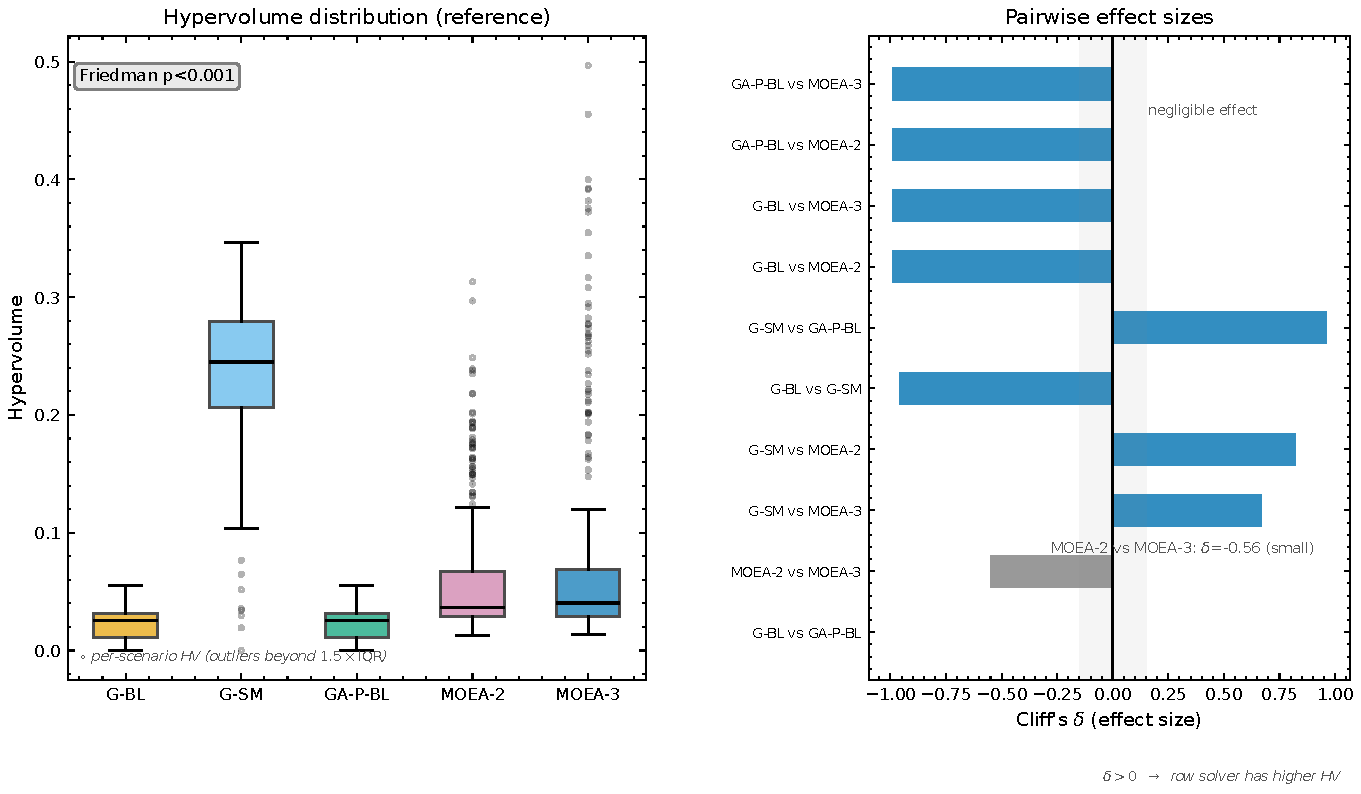
\includegraphics[width=\textwidth]{fig1_hypervolume.pdf}
    \caption{统计验证：（左）超体积分布；（右）配对 Cliff's $\delta$ 效应量。灰色波段标记可忽略效应（$|\delta|<0.147$）。}
    \label{fig:fig4}
\end{figure}

如图~\ref{fig:fig4} 所示，上述求解器比较经超体积分布与配对 Cliff's $\delta$ 效应量统计验证。
以下各节从五个角度深化这一总体分析：\S\ref{sec:squint-special} 聚焦斜视感知调度的特殊权衡，
\S\ref{sec:scale-sensitivity} 考察尺度敏感性（多目标优势如何随目标密度变化），
\S\ref{sec:pareto-coupling} 揭示帕累托压缩的几何机制，
\S\ref{sec:ablation} 通过消融验证该机制的条件依赖，
\S\ref{sec:robustness-calibration} 则通过鲁棒性控制分离初始化与搜索预算的混淆效应。

% ── 6.2 斜视感知特殊区域 ──
\subsection{斜视感知特殊区域}
\label{sec:squint-special}
最小化斜视贪心求解器（G-SM）通过在每个可见窗口内选择最小化斜视角的观测时间，
相对于仅收益基线（G-BL）改善了 NESZ 辐射质量（$f_3$）。
在所有 200 个场景中，这对 $f_3$ 产生了大正效应
（Cliff's $\delta = +0.91$, $p < 10^{-34}$），覆盖率成本较大
（Cliff's $\delta = -1.0$, $p < 10^{-34}$，在原始 $f_1$ 上；此处用原始 $f_1$ 因为 G-BL 的定义给出恒定 $f_1^* = 1.0$，归一化利润比较退化为对固定值的一样本检验）。
然而，这种权衡强烈依赖于密度。
在稀疏场景（S1, $N = 20$）中，G-SM 降至 $f_1^* = 0.51 \pm 0.16$
（相对于 G-BL 的 $1.00$ 下降 $-49\%$），同时将 $f_3$ 从 $0.271 \pm 0.057$ 提高到 $0.644 \pm 0.058$（$+138\%$）。
在密集场景（S4, $N = 500$）中，$f_1$ 成本升级：
G-SM 实现 $f_1^* = 0.37 \pm 0.12$（$-63\%$），$f_3$ 从 $0.53 \pm 0.11$ 上升到 $0.700 \pm 0.058$（$+32\%$）。
图~\ref{fig:fig1} 可视化这种密度依赖的权衡：面板 (c) 中的 LOESS 趋势识别了 $N = 100$ 附近的过渡区域，
其中 $f_1$ 惩罚快速增长。
辐射优势随密度收窄（从 S1 的 $+138\%$ 到 S4 的 $+32\%$），因为紧密排列的时间窗口限制了每次获取向斜视最小化时刻移动的程度；
而覆盖率成本在每个密度下都保持较大（G-SM 排定的任务至多为 G-BL 选择的 $44\%$，在 $N \geq 100$ 时降至约 $20$--$27\%$）。
\begin{figure}[H]
    \centering
    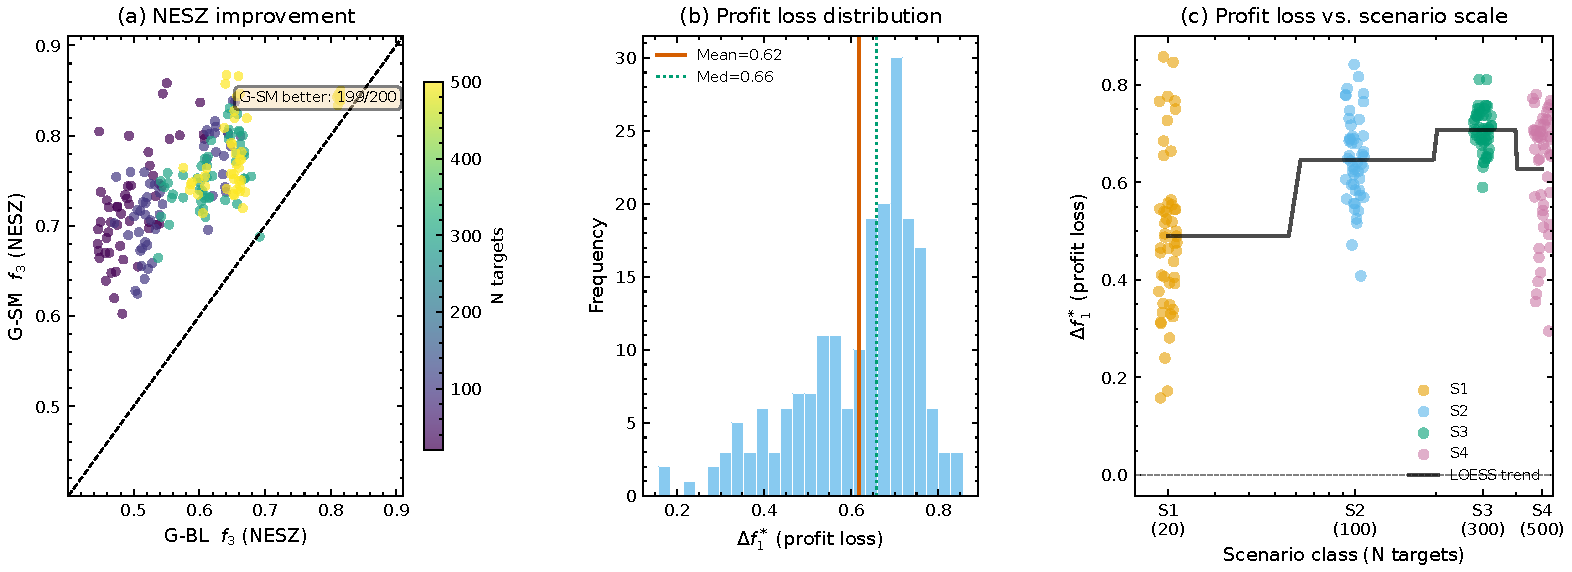
\includegraphics[width=\textwidth]{fig2_squint_effect.pdf}
    \caption{斜视感知调度的效果：(a) $f_3$ 散点图；(b) $\Delta f_1^*$ 直方图；(c) $\Delta f_1^*$ 与 $N$ 的关系及 LOESS 趋势}
    \label{fig:fig1}
\end{figure}

% ── 6.3 尺度敏感性（图 5）──
\subsection{尺度敏感性}
\label{sec:scale-sensitivity}
MOEA-2 与 G-BL 之间的差距随目标密度系统性地变化（图~\ref{fig:fig5}，表~\ref{tab:scale-sensitivity}）。
MOEA-2 相对于 G-BL 的覆盖率差距仅限于稀疏密度：
从 S1（$N = 20$）的 $f_1^* = 0.87 \pm 0.08$ 升至 S2（$N = 100$）的 $0.985 \pm 0.03$，
在 $N \geq 150$（S7--S3）达到 $0.998$--$0.999$，并在 S4（$0.996$）保持 G-BL 的 $1\%$ 以内。
$f_2$ 相对于 G-BL 的改进同步收缩，从 $+4.7\%$（S1）降到 $+1.4\%$（S2），在 $N \geq 150$ 时不高于 $+0.8\%$。
MOEA-2 覆盖率显著低于 G-BL 的场景比例（$f_1^* < 0.95$，即覆盖率差距超过 5\%）
从 $84\%$（S1）骤降至 $6\%$（S2），并在 $N \geq 150$ 时为 $0\%$（S4 为 $2\%$，仅一个场景）。
因此多目标覆盖优势是稀疏密度现象：在 $N = 20$ 到 $N = 100$ 之间，
求解器从主动以覆盖率换取质量转变为在贪心基线附近运行，超过 $N = 150$ 后差距实际上为零。
\begin{figure}[H]
    \centering
    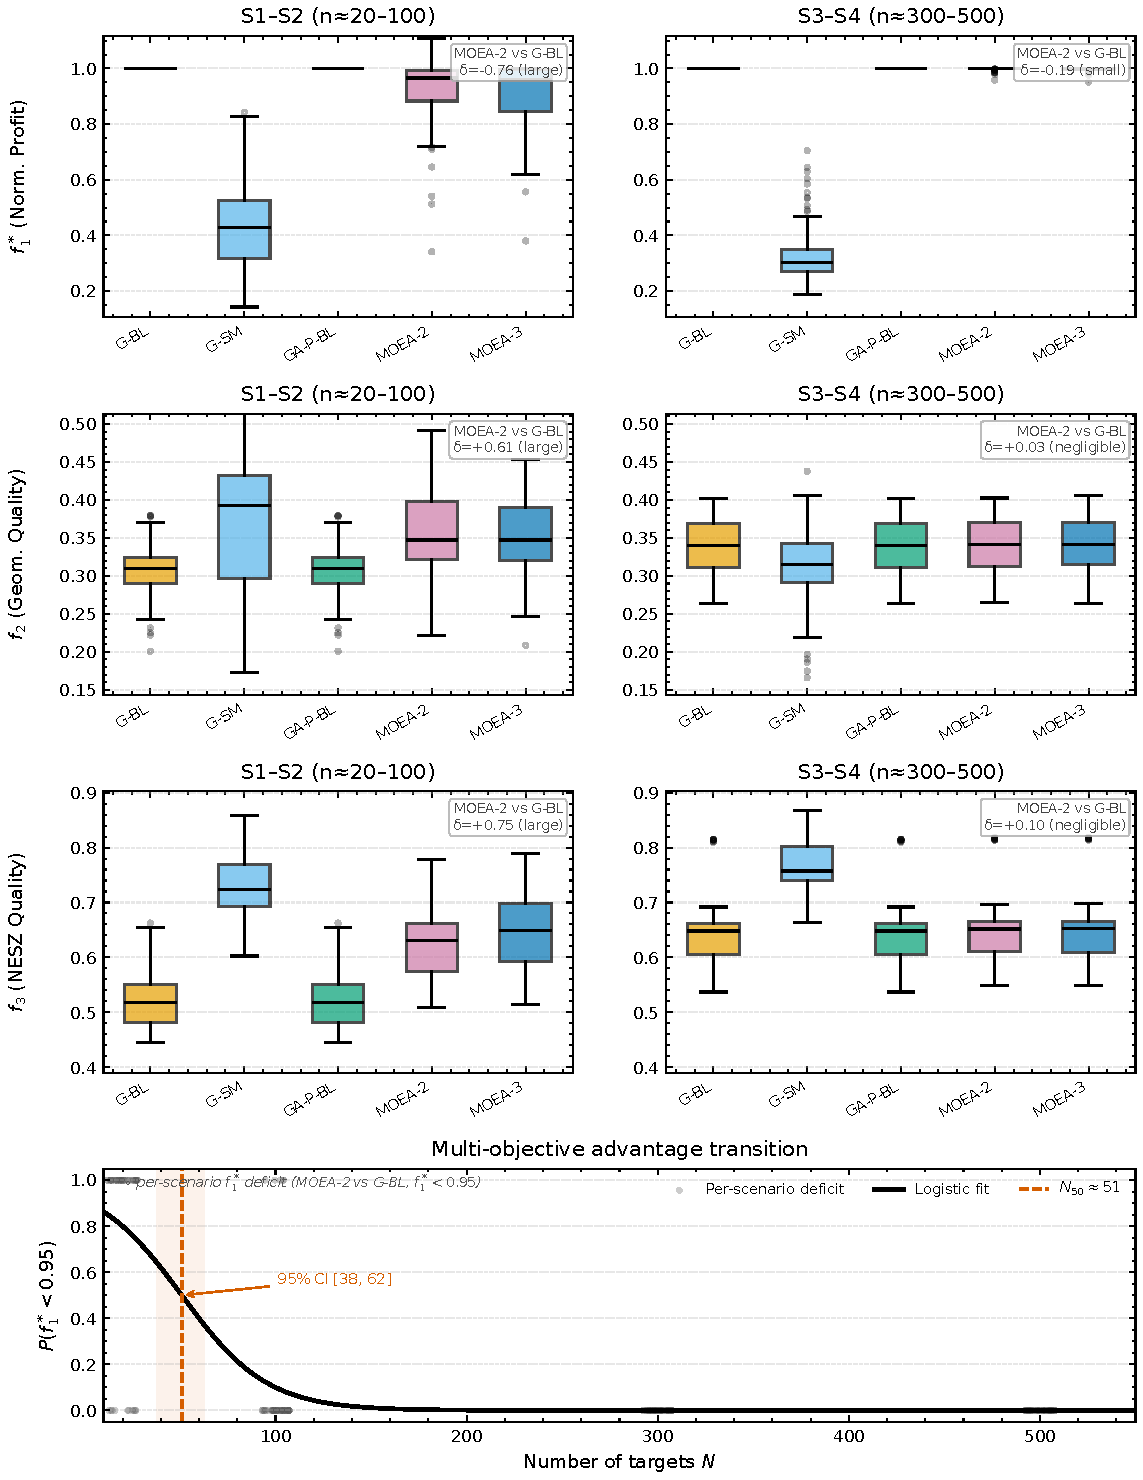
\includegraphics[width=0.75\textwidth]{fig3_scale_sensitivity.pdf}
    \caption{按场景组和求解器划分的几何质量（$f_2$）}
    \label{fig:fig5}
\end{figure}
\begin{table}[H]
\centering
\caption{MOEA-2 vs. G-BL 的尺度敏感性}
\label{tab:scale-sensitivity}
\begin{tabular}{lcccc}
\toprule
\textbf{类别} & $N$ & $f_1^*$（MOEA-2） & $f_2$ 改进 & \% $f_1^* < 0.95$ \\
\midrule
S1 & 20   & $0.87 \pm 0.08$ & +4.7\% & 84\% \\
S2 & 100  & $0.985 \pm 0.03$ & +1.4\% & 6\% \\
S7 & 150  & $0.998 \pm 0.00$ & +0.8\% & 0\% \\
S8 & 200  & $0.997 \pm 0.01$ & +0.7\% & 0\% \\
S3 & 300  & $0.999 \pm 0.00$ & +0.6\% & 0\% \\
S4 & 500  & $0.996 \pm 0.01$ & +0.5\% & 2\% \\
\bottomrule
\end{tabular}
\end{table}
对 $f_1^* < 0.95$ 的场景比例拟合逻辑回归 $p(\text{deficit} \mid N) = 1 / (1 + \exp(-(\alpha + \beta N)))$
得出过渡中点 $N_{50} \approx 50$ 个目标。
该估计弱约束：只有两个稀疏密度（$N=20, 100$）携带信息性差距比例（$84\%$ 和 $6\%$），
而四个更密集的点都不超过 $2\%$，因此 bootstrap 置信区间不收敛。
$N_{50}$ 应被视为"过渡限于 $N \in [20, 100]$"的粗略指示，而非精确阈值。
超过 $N \approx 150$ 后，没有任何场景显示超过 $5\%$ 的覆盖率差距（比例为 $0\%$）。

% ── 6.4 帕累托压缩机制 ──
\subsection{帕累托压缩机制}\label{sec:pareto-coupling}

本节从两个现象和一个机制的角度分析帕累托前沿的结构。

现象一：前沿压缩。图~\ref{fig:fig2} 可视化了代表性 S4 场景上的帕累托前沿。
前沿包含 $20.5 \pm 9.9$ 个 MOEA-3 非支配解（MOEA-2: $1.8 \pm 1.0$），
但是压缩的：仅跨越约 $0.06$ 的 $f_1^*$ 和 $0.003$ 的 $f_2$，
而稀疏 S1 场景中 $\Delta f_2 \approx 0.12$，确认了
\S\ref{sec:scale-sensitivity} 中记录的尺度依赖饱和。
在密集目标区域中，求解器收敛到低斜视几何加上调度饱和限制了质量分化，
与求解器策略无关。在此密度下 MOEA-2 与 MOEA-3 前沿几乎重合，
表明在密集设置中添加 $f_3$ 作为第三目标仅产生极小的额外区分度。

\begin{figure}[H]
    \centering
    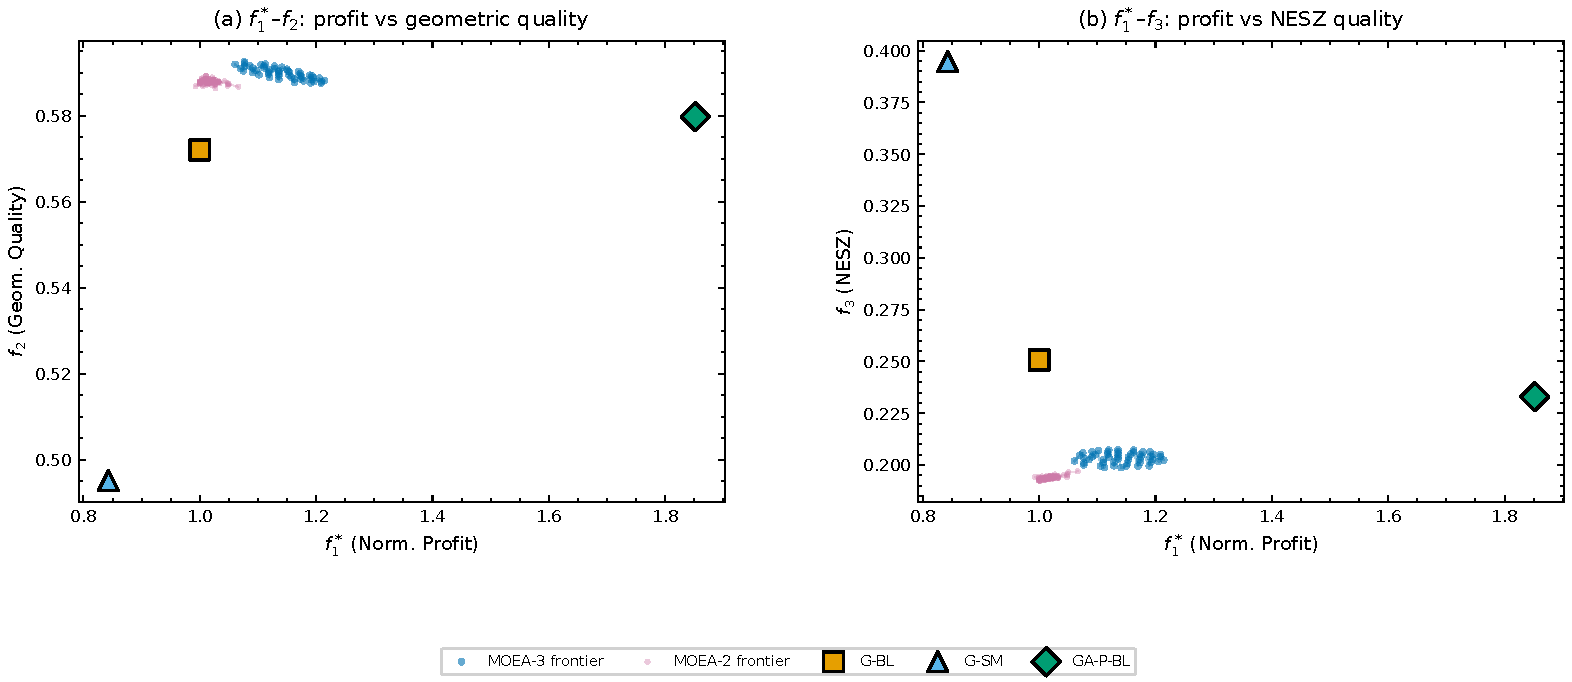
\includegraphics[width=0.75\textwidth]{fig4_solver_profiles.pdf}
    \caption{代表性 S4 场景（$N=500$）上的帕累托前沿：MOEA-3 前沿叠加 MOEA-2 和基线求解器标记。面板 (a): $f_1^*$--$f_2$；面板 (b): $f_1^*$--$f_3$。}
    \label{fig:fig2}
\end{figure}

$f_1^*$--$f_2$ 投影（面板 a）显示极度压缩的曲面：
即使对于 $f_1^*$ 展布最宽的 S4 场景，前沿也仅跨越 $f_1^* \in [0.94, 1.00]$ 和 $f_2 \in [0.500, 0.503]$
——全覆盖处的近垂直线段。
叠加单点基线解显示 G-BL 位于前沿的"全覆盖、中等质量"角落，
而 G-SM 占据定性不同的区域（$f_1^* \approx 0.37$, $f_3 \approx 0.70$），
位于 MOEA-3 帕累托曲面之外——这是 G-SM 激进斜视最小化的结果。

现象二：密度依赖的第三目标价值。
MOEA-3 与 MOEA-2 的差异强烈依赖密度：在 S1，含物理目标的求解器达到 $f_3 = 0.428\pm0.064$，
而 MOEA-2 为 $0.233\pm0.027$（$+84\%$），代价是 $f_2$ 约 $10\%$（$0.540\pm0.021$ vs.\ $0.600\pm0.021$）；
在 S4，$f_3$ 优势骤降至 $+1.5\%$（$0.535\pm0.109$ vs.\ $0.527\pm0.111$），$f_2$ 代价可忽略。
第三目标因此在稀疏密度下**并非冗余**——此时覆盖率压力低，求解器可自由以 $f_2$ 换取 $f_3$——
但在运营密度下优势消失，因为覆盖率压力锁定了选择，而非底层 $f_2$--$f_3$ 权衡消失——
调度内相关性实际上随密度**增强**（\S~\ref{sec:pareto-coupling}）。

HV 排序（表~\ref{tab:hv}）与覆盖率排序（表~\ref{tab:solver-profiles}）的差异进一步说明了这一点：
在表中三个求解器内，G-BL 在覆盖率（$f_1^*$）上排名第一但在 HV 上排名第三，
而 NSGA-III 变体在 HV 上排名前二（MOEA-3 第一，MOEA-2 第二）。
这种反转源于点计数不对称：单目标求解器各贡献一个点，而 MOEA-3 在 S1 贡献 $53.3 \pm 6.7$ 个非支配解
（MOEA-2: $7.3 \pm 2.6$），这一基数差距在 S3--S4 依然存在（虽较轻微）。
因此 HV 对点计数而非解质量敏感——但前沿压缩才是核心现象，而非点的数量。
\label{sec:hv-divergence}

机制：几何耦合与低斜视收敛。

由于 $\theta$ 和 $\psi_{\text{sq}}$ 并非独立，而是均源自同一 LOS 向量 $\mathbf{l} = (l_x, l_y, l_z)$
（\S~\ref{sec:system-model}），每任务的 $f_2$ 和 $f_3$ 贡献共享几何结构。
为分离定义性耦合与调度器诱导的相关性，我们计算解析零分布，
将观测几何视为从可达包络（$\theta \in [15^\circ, 50^\circ]$, $|\psi_{\text{sq}}| \leq 45^\circ$）中均匀随机抽取，
并封闭形式地评估 $f_{2,i} = \sin\theta_i \cos\psi_{\text{sq},i}$ 和 $f_{3,i} = \cos^3\theta_i \cos^3\psi_{\text{sq},i}$ 的矩积分
（经蒙特卡洛验证，$r_{\text{MC}} = -0.5120$, $N = 2\times10^5$）。
零相关性为
\begin{equation}
r_{\text{null}} = \frac{\mathrm{Cov}(f_2, f_3)}{\sqrt{\mathrm{Var}(f_2)\,\mathrm{Var}(f_3)}} \;=\; -0.51,
\label{eq:rnull}
\end{equation}
其中零假设下 $\theta$ 和 $\psi_{\text{sq}}$ 的独立性将矩分解为因子形式，
例如 $E[f_2 f_3] = E[\sin\theta\cos^3\theta]\,E[\cos^4\psi_{\text{sq}}]$。
负号揭示了一种结构性冲突，而非冗余：在仅 $\theta$ 极限（固定斜视）下，
$f_{2,i} \propto \sin\theta$ 与 $f_{3,i} \propto \cos^3\theta$ 严格反单调
（$r_\theta = -0.997$），因为 $f_2$ 偏好高入射角而 $f_3$ 偏好低入射角；
在仅 $\psi_{\text{sq}}$ 极限（固定 $\theta$）下，两者均正依赖于 $\cos\psi_{\text{sq}}$
（$r_\psi = +0.997$），因为低斜视对两者都有利。
在均匀几何下，$\theta$ 冲突占主导，产生 $r_{\text{null}} < 0$。

\textit{经验相关性与低斜视收敛。}
在全部 200 个场景的调度任务上池化后，求解器选择的调度内的逐任务经验相关性
$f_2$ 与 $f_3$ 之间在每个密度下均为负，且随密度升高而**增强**：
完整物理模型（变体 A）从 $-0.61$（S1）到 $-0.78$（S4），
无物理变体 D 从 $-0.56$（S1）到 $-0.78$（S4）。
因此 $\theta$ 冲突在调度内部仍然存在，而非被反转。
所有求解器都选择了低斜视几何，使 $f_2$ 与 $f_3$ 沿共享的 $\cos\psi_{\text{sq}}$ 因子对齐，
并在稀疏密度下最强地衰减包络相关性（S1 处 $-0.97 \to -0.61$）；
随着密度升高，覆盖率压力迫使调度纳入更宽入射角范围的任务，拓宽 $\theta$ 展布并增强残差负相关
（平均 $f_2$ 从 S1 的 $0.54$ 降至 S4 的 $0.51$，平均 $f_3$ 从 $0.43$ 升至 $0.52$）。
三目标冗余因此是一种经验收敛效应——并非 $f_2$ 与 $f_3$ 之间的数学恒等关系，
而是覆盖率压力在高密度下移除交易自由的结果，入射角冲突本身依然存在。

\textit{包络相关性与调度相关性的对比。}
包络相关性与调度相关性形成鲜明对比。
在 C1 可行包络（$|\psi_{\text{sq}}| \leq 45^\circ$；在 20 个场景（S1--S4 每密度类 5 个，取最小种子编号）的全部可见窗口中，
以 10 秒为离散步长，约 $3.9 \times 10^5$ 个窗口-时间步对）中，
$\mathrm{corr}(f_2, f_3) = -0.97$，由入射角冲突主导的强负相关。
相比之下，求解器选择的调度将该相关性向零移动——从包络的 $-0.97$ 变为完整物理调度内的
$-0.61$（S1）——但并未反转其符号：低斜视收敛衰减了入射角冲突，而非消除它。
这种部分衰减是求解器的主动效果，而非几何包络约束的结果：
如果只是约束限制了可行几何，相关性应保持负值（接近 $-0.97$）。
消融研究独立支持了这一解释。移除全部物理目标后（变体 D，\S~\ref{sec:ablation}），
S1 的调度级相关性为 $r \approx -0.56$——比含物理的变体 A（$r \approx -0.61$）更接近零——
而两类变体在高密度下收敛到相同的强负水平（S4 时 $r \approx -0.78$）。
稀疏区域中，物理目标保留遍历 $f_2$--$f_3$ 质量权衡的解，维持略强的残差负相关；
移除物理目标后，求解器仅最大化覆盖，时间紧凑性偶然偏好低斜视窗口，进一步削弱了残差相关。
高密度下这种结构性紧凑性主导，与目标形式无关，故消融对比消失，
相关性饱和于强负水平；第三目标的价值丧失并非因为冲突减弱，
而是因为任何目标形式都无法逃脱覆盖率驱动的 $\theta$ 展布。
与这种尺度依赖饱和一致，逐密度超体积在高密度下收缩：S4 的池化 HV 为其 S1 值的
$0.18$（MOEA-2）与 $0.11$（MOEA-3），即 S4/S1 超体积比远小于 1，
反映 \S~\ref{sec:pareto-coupling} 记录的前沿压缩（S4 前沿仅跨越 $\Delta f_1^* \approx 0.06$）而非退化。
我们提醒，此处报告的帕累托前沿是通过 NSGA-III 获得的最佳已知近似；
它们是否代表真实帕累托最优集，在没有精确方法（如 MILP 或分支定界）的情况下是未知的，
而精确方法对于此问题类别中 $N \geq 20$ 的情况仍然难以处理。

% ── 消融研究（物理建模的贡献） ──
\subsection{物理建模的消融研究}
\label{sec:ablation}

为了量化入射角（$\theta$）与斜视角（${\psi_{\text{sq}}}$）建模对求解器性能的贡献，
我们使用四种目标函数变体重复了 MOEA-3 实验：
%
\begin{description}
\item[A. 完整物理模型（基线）] $f_2 = \frac{1}{|\mathcal{S}|}\sum \sin\theta_{\text{elev},i} \cdot \cos\psi_{\text{sq},i}$，
      $f_3 = \frac{1}{|\mathcal{S}|}\sum \cos^3\xi_i$
      （与 \S~\ref{sec:pareto-coupling} 中的标准配置相同）。
\item[B. 去除斜视分量] $f_2 = \frac{1}{|\mathcal{S}|}\sum \sin\theta_{\text{elev},i}$，
      $f_3 = \frac{1}{|\mathcal{S}|}\sum \cos^3\theta_{\text{elev},i}$（移除 ${\psi_{\text{sq}}}$ 分量；
      $\theta_{\text{elev}}$ 为高程面入射角，$\cos\theta_{\text{elev}}=\cos\xi/\cos\psi_{\text{sq}}$）。
\item[C. 去除入射角分量] $f_2 = \frac{1}{|\mathcal{S}|}\sum \cos\psi_{\text{sq},i}$，
      $f_3 = \frac{1}{|\mathcal{S}|}\sum \cos^3\psi_{\text{sq},i}$（移除 $\theta_{\text{elev}}$ 分量）。
\item[D. 不含物理信息] $f_2 = f_3 = 1$（逐任务的目标为常数；求解器不接收
      任何几何信息；表~\ref{tab:ablation} 中所示的 $f_2$、$f_3$
      为基于所得调度结果实际观测几何事后计算的诊断值）。
      变体 D 充当零模型对照：它检验 NSGA-III 求解器的性能应归因于 $f_2$ 和 $f_3$
      的物理内容，还是仅仅归因于结构化搜索的附加目标的存在。
\end{description}
%
四种变体均使用相同的 NSGA-III 参数（种群大小 $= 100$，
代数 $= 200$，Das--Dennis $p=12$）、相同的场景文件，
以及相同的 G-BL 热启动注入。仅目标函数不同，
因此本实验属于受控消融，而非重新调参实验。
在相同 NSGA-III 参数与相同 G-BL 种子注入下的求解器内消融充分控制了混淆因素，
使得 Wilcoxon 符号秩检验适用于目标函数变体的配对比较。
每种变体完成 6 个场景类别 $\times$ 50 个随机种子 $= 300$ 次运行
（A--D 共计 1,200 次运行）；表~\ref{tab:ablation} 报告密度区间类别 S1--S4。
其余两个类别施压于非密度轴：S5 保持 $N=20$ 密度但将目标位置沿轨散布于
$5^\circ$/$15^\circ$/$25^\circ$/$35^\circ$/$45^\circ$（斜视散布灵敏度组），
S6 将 20 个目标打包为 2--10 个窄窗簇（窗口宽 60--180 秒；C3 转换应力组）。
退化指标定义为
$\Delta\% = (\text{A} - \text{V})/\text{A} \times 100$，
其中 A 为完整物理基线，V 为待比较变体；
负值表示变体在 $f_1^*$ 上优于基线。

\begin{table}[H]
\centering
\caption{各场景类别下的消融结果。加粗：$p < 0.005$（与 A 配对 Wilcoxon 符号秩检验；与 \S\ref{sec:evaluation-metrics} 的 Friedman--Wilcoxon 框架一致）。}
\label{tab:ablation}
\begin{tabular}{llccccrc}
\toprule
\textbf{类别} & \textbf{V} & \textbf{$f_1^*$} & \textbf{$f_2$} &
\textbf{$f_3$} & \textbf{$f_1/n$} & \textbf{$n_\text{sel}$} &
\textbf{$\Delta f_1^*\%$} \\
\midrule
\multirow{4}{*}{S1 ($N=20$)}
 & A & $0.850 \pm 0.123$ & $0.376$ & $0.698$ & $5.99 \pm 0.73$ &
   $15.6 \pm 2.6$ & (基线) \\
 & B & $0.852 \pm 0.152$ & $0.353$ & $0.574$ & $6.01 \pm 0.83$ &
   $15.7 \pm 3.1$ & $-0.8\%$ \\
 & C & $0.845 \pm 0.095$ & $0.375$ & $0.703$ & $5.86 \pm 0.80$ &
   $16.0 \pm 2.2$ & $+0.1\%$ \\
 & D & $1.002 \pm 0.011$ & $0.302$ & $0.525$ & $5.65 \pm 0.66$ &
   $19.5 \pm 0.7$ & $\mathbf{-18.0\%}$ \\
\midrule
\multirow{4}{*}{S2 ($N=100$)}
 & A & $0.976 \pm 0.040$ & $0.329$ & $0.597$ & $5.58 \pm 0.42$ &
   $62.7 \pm 19.3$ & (基线) \\
 & B & $0.990 \pm 0.022$ & $0.321$ & $0.570$ & $5.55 \pm 0.37$ &
   $63.6 \pm 19.1$ & $\mathbf{-1.2\%}$ \\
 & C & $0.977 \pm 0.033$ & $0.328$ & $0.599$ & $5.57 \pm 0.40$ &
   $62.8 \pm 19.3$ & $+0.0\%$ \\
 & D & $1.000 \pm 0.000$ & $0.317$ & $0.562$ & $5.54 \pm 0.37$ &
   $64.2 \pm 18.8$ & $\mathbf{-2.0\%}$ \\
\midrule
\multirow{4}{*}{S3 ($N=300$)}
 & A & $0.998 \pm 0.005$ & $0.344$ & $0.623$ & $5.63 \pm 0.30$ &
   $154.2 \pm 39.9$ & (基线) \\
 & B & $0.998 \pm 0.005$ & $0.343$ & $0.618$ & $5.63 \pm 0.29$ &
   $154.2 \pm 40.0$ & $+0.0\%$ \\
 & C & $0.998 \pm 0.004$ & $0.344$ & $0.623$ & $5.63 \pm 0.30$ &
   $154.2 \pm 39.9$ & $+0.0\%$ \\
 & D & $1.000 \pm 0.000$ & $0.342$ & $0.616$ & $5.63 \pm 0.29$ &
   $154.5 \pm 39.9$ & $\mathbf{-0.2\%}$ \\
\midrule
\multirow{4}{*}{S4 ($N=500$)}
 & A & $0.997 \pm 0.008$ & $0.338$ & $0.680$ & $5.83 \pm 0.44$ &
   $142.3 \pm 72.1$ & (基线) \\
 & B & $0.999 \pm 0.003$ & $0.337$ & $0.677$ & $5.84 \pm 0.44$ &
   $142.5 \pm 72.0$ & $-0.1\%$ \\
 & C & $0.998 \pm 0.006$ & $0.337$ & $0.680$ & $5.83 \pm 0.44$ &
   $142.4 \pm 72.0$ & $+0.0\%$ \\
 & D & $1.000 \pm 0.000$ & $0.336$ & $0.675$ & $5.83 \pm 0.45$ &
   $142.7 \pm 71.9$ & $\mathbf{-0.2\%}$ \\
\bottomrule
\end{tabular}
\end{table}

\begin{figure}[H]
    \centering
    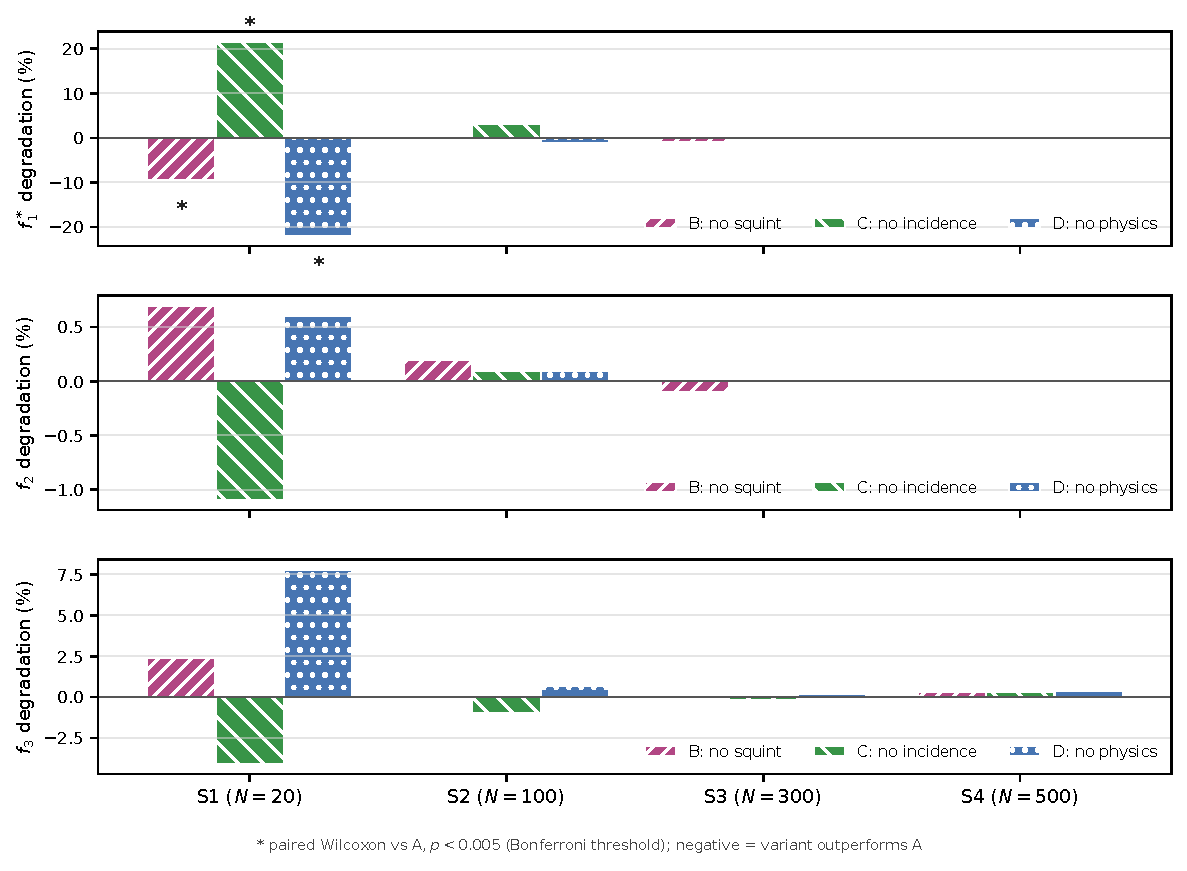
\includegraphics[width=\textwidth]{fig5_ablation.pdf}
    \caption{四种目标函数变体（B--D）与四类场景（S1--S4）下的消融结果。柱状图表示相对完整物理基线 A 的归一化收益 $f_1^*$ 与事后几何质量指标 $f_2$、$f_3$ 的退化（负值表示变体优于 A）；星号标记与 A 配对 Wilcoxon 比较 $p<0.005$（Bonferroni 阈值）。}
    \label{fig:fig5}
\end{figure}

表~\ref{tab:ablation} 与图~\ref{fig:fig5} 中的消融结果表明，物理目标建模的影响
集中在稀疏场景中，并随场景密度的增大而消失 ---
这与我们的尺度敏感性分析（\S~\ref{sec:scale-sensitivity}）模式一致。

在 S1（$N = 20$）下，仅变体 D（不含物理信息）在本文 $p<0.005$ 阈值下
与基线 A 存在显著差异：其 $f_1^*$ 升至 $1.002$（$-18.0\%$，$p=3.4\times10^{-9}$），
通过多调度 $3.9$ 个任务（$19.5$ vs.\ $15.6$），代价是事后 $f_3$ 从 $0.698$
降至 $0.525$（$-25\%$）。变体 B（去除斜视）使 $f_1^*$ 基本不变（$-0.8\%$，$p=0.46$），
但将 $f_3$ 降至 $0.574$（$-18\%$）、$f_2$ 降至 $0.353$（$-6.2\%$，$p=1.1\times10^{-5}$）：
缺少斜视惩罚后求解器容忍更高的斜视视角，牺牲了完整物理基线在稀疏区域购买的辐射质量。
变体 C（去除入射角分量）在报告的任何指标上均无可测变化。
这种惰性与窗口几何一致：高程面入射角在一个可见性窗口内仅变化几度（S1 场景中均值约 $1.5^\circ$），
而斜视角扫过约 $20$--$35^\circ$，因此 $f_2$/$f_3$ 中的 $\theta_{\text{elev}}$ 因子在每个窗口内近似为共同尺度；
移除它保持了窗口内任务排序，从而保持了选中的调度。
\S\ref{sec:pareto-coupling} 的入射角冲突因此通过跨窗口/聚合几何起作用，而非通过窗口内选择。
因此，物理目标的内容在稀疏区主要通过辐射质量（$f_3$）与完全移除时的覆盖率反差影响结果，
而仅移除任一几何分量均不改变覆盖率。

到 S2（$N = 100$）时，变体 B 与 D 仍与 A 显著不同但效应很小
（$-1.2\%$，$p=5.3\times10^{-4}$ 与 $-2.0\%$，$p=1.7\times10^{-6}$）：
移除斜视或全部物理信息仍会适度改变覆盖率。变体 C 仍与 A 无法区分。

在 S3--S4（$N \geq 300$）下，每种变体在 $f_1^*$ 上均落在基线 $0.2\%$ 以内，
在 $f_2$ 上均在 $0.6\%$ 以内；D 的配对检验显著性反映的是一致但可忽略的效应（$-0.2\%$）。
这种数值不变性正是 \S~\ref{sec:scale-sensitivity} 中讨论的
尺度依赖饱和的直接表征：一旦候选观测窗口的密度饱和了调度，
目标函数便仅惩罚不可行的解，而不再区分可行的解。
在此情形下，无论 $f_2$ 与 $f_3$ 是否承载几何含义（A），
还是充当常数占位符（D），NSGA-III 求解器
本质上等价于一种约束过滤下的收益最大化器。

两个稳健性类别在密度轴之外复制了该模式。在 S5（沿轨目标散布）和 S6（窄窗簇）上，
完全移除变体 D 在 $f_2$ 上显著差于 A（$-11.2\%$，$p=1.6\times10^{-13}$ 和 $-11.1\%$，$p=1.8\times10^{-15}$）、
在 $f_3$ 上同样更差（$-6.1\%$ 和 $-6.3\%$），C 与 A 不可区分（$f_2$ $+0.4\%$，$p=0.33$ 和 $-0.6\%$，$p=0.48$），
B 呈现小幅显著差异（$f_2$ $+3.2\%$，$p=0.046$ 和 $+4.6\%$，$p=1.2\times10^{-5}$）。
物理目标的覆盖率代价在此同样持续：D 比 A 多获得 $17\%$（S5）和 $8\%$（S6）的原始收益，
即在稀疏配置下目标驱动的选择无论施压轴是密度、目标散布还是窗口簇都会牺牲覆盖率。

综合来看，物理质量目标主要在稀疏区域增加价值，且主要通过辐射质量：
在 S1，完整物理变体 A 相比无物理变体 D 实现 $f_3$ 的 $33\%$ 提升（$0.698$ vs.\ $0.525$；在共同退化基线上 D 比 A 低 $25\%$），
代价是 $18\%$ 覆盖率劣势；仅移除斜视分量（B）已在保持 $f_1^*$ 的同时牺牲 $18\%$ 的 $f_3$。
部分移除目标的覆盖率效应在所有区间均极小，且到 $N \geq 300$ 时
物理目标的选择对结果数值上不再有影响。


% ── 6.6 鲁棒性与校准 ──
\subsection{鲁棒性与校准}
\label{sec:robustness-calibration}
上述机制必须与初始化和搜索预算效应分离。因此我们使用四个控制实验。

\paragraph{热启动依赖性.}
在 10 个 S1、4 个 S2、5 个 S3 和 5 个 S4 场景上（每个 3 个种子），随机初始化 MOEA-2 的 $f_1^*$ 差距
分别约为 $-0.245 \pm 0.107$、$-0.486 \pm 0.071$、$-0.678 \pm 0.020$ 和 $-0.540 \pm 0.042$
（各次运行的均值 $\pm$ 标准差），相对于热启动 MOEA-2。
因此，G-BL 种子在每个测试密度上实质性改善覆盖率收敛；值得注意的是，该差距在最密集的 S3 类最大，
而非最稀疏的类，表明高目标密度本身并不使随机初始化充分。
这限定了覆盖上限的主张：接近 G-BL 是初始化依赖的。
相比之下，随机初始化的 $f_2$ 在各密度几乎不变（S3 为 $0.549$ 对 $0.551$，S4 为 $0.551$ 对 $0.551$），
因此低斜视区间并非锚点伪像；覆盖差距仅局限于 $f_1^*$。
覆盖收敛到 G-BL 因而是初始化效应，而非 MOEA 框架本身的伪像。

\paragraph{扰动敏感性.}
在 MOEA-3 上对 $\sigma\in\{0.1,0.3,0.5,0.7\}$ 进行扫描（每个值 10 个 S3 场景，固定求解器种子）
使 $f_2$ 与 $f_3$ 的均值基本不变（各水平均值 $f_2 = 0.5492$、$f_3 = 0.1401$，水平间变化低于 $10^{-3}$），
覆盖率恒为 $200/300$ 选中任务。
\S~\ref{sec:pareto-coupling} 中报告的逐任务 $f_2$--$f_3$ 耦合因而是调度几何的属性，而非扰动幅度的属性，
三目标冗余在 $\sigma=0.1$--$0.7$ 范围内持续，不是 $\sigma=0.5$ 扰动水平的伪像。

\paragraph{随机搜索校准.}
在五个 S1 场景上，每个场景 5,000 次随机任务选择产生均值 $f_1^*=0.527\pm0.003$，
第 90 百分位 $0.930\pm0.008$；最佳样本达到 $1.000$——即 G-BL 利润，
随机采样最多只能复现贪心基线，而无法超过它。
随机抽样仅凭偶然达到高覆盖，MOEA 的增益因此反映结构化搜索而非运气。

\paragraph{随机初始化控制.}
随机初始化的变体 D 控制（15 个 S3 和 15 个 S4 运行，无 G-BL 热启动）
也收敛到低斜视，S3 和 S4 的 $f_2=0.551\pm0.001$——略高于（更低的斜视）热启动的 D 求解器
（$f_2\approx0.515$--$0.535$），因此低斜视收敛是目标内在的，而非热启动残留：
G-BL 种子在最早可行时刻插入任务，从而将热启动运行偏向贪心调度的更高斜视。
A--D 不变性本身在标准预算下已然成立（表~\ref{tab:ablation}：S3--S4 处 $\Delta f_1^* \leq 0.1\%$），
这是覆盖率压力在高密度下锁定选择的物理必然结果（\S~\ref{sec:pareto-coupling}）；
该收敛因而不是预算伪像。
这些控制共同支持低斜视收敛解释，排除了热启动残留、噪声水平敏感性或随机偶然性的替代解释，同时不排除所有算法特定效应。

% ============================================================
%  7. 讨论
% ============================================================
\section{讨论}
% ── 7.1 发现总结与运营指导意义 ──
\subsection{发现总结}
\label{sec:summary}
我们将一个求解器在尺度 $N$ 上定义为 \emph{帕累托充分的}，如果比较集合中没有替代求解器
在统计显著（$p < 0.005$, Cliff's $|\delta| > 0.33$）的条件下同时实现更高的 $f_1^*$ 和更高的 $f_2$（或 $f_3$）。
这一操作标准区分了多目标优化产生可测量质量-覆盖优势的情况和它不产生优势的情况。
在窗口修正后的数据下，即使在最稀疏密度也没有求解器达到帕累托充分：
在 $N=20$ 处三个维度构成一个真实的权衡曲面——G-BL 保持最高的 $f_1^*$（$1.00$）和中等 $f_3$（$0.271$），
MOEA-2 达到最高的 $f_2$（$0.600$）但 $f_3$ 最低（$0.233$），
MOEA-3 以 $f_2$（相对 MOEA-2 约 $-10\%$）换取最高的 $f_3$（$0.428$，相对 MOEA-2 $+84\%$）——
因此没有求解器在一个以上维度占优，
而在 $N \geq 300$ 时所有求解器收敛到 G-BL 锚点，贪心基线在操作上充分。
我们的实验跨越 200 个系统变化的场景，产生了五个相互关联的发现。

\textbf{(1)}~多目标优化的质量优势随目标密度饱和：
$f_2$ 改进从 $N=20$ 的 $+4.7\%$ 缩小到 $N=500$ 的 $+0.5\%$。
显示覆盖率差距（$f_1^* < 0.95$）的场景比例从 $84\%$ 骤降至 $2\%$（表~\ref{tab:scale-sensitivity}）。
在运营密度（$N \gtrsim 300$）下，以 G-BL 为种子的 MOEA-2 和 MOEA-3 公式化接近 G-BL 覆盖锚点，
边际几何质量增益可忽略。
GA-P-BL 的输出与 G-BL 完全相同（其"不劣于基线"保护在单一利润目标上总是触发），
因此收敛主张涉及添加物理目标的边际价值，而非所有面向收益求解器的通用上限。


\textbf{(2)}~第三目标是密度依赖的而非冗余的：
调度内的逐任务 $f_2$--$f_3$ 相关性在每个密度下均为负且随密度**增强**
（全物理求解器约 $-0.61$ 至 $-0.78$；\S~\ref{sec:pareto-coupling}），
并且 MOEA-3 在稀疏密度于 $f_3$ 上与 MOEA-2 分离（$N=20$ 处 $+84\%$）而优势在 $N \geq 300$ 缩小至约 $+1.5\%$，
确认入射角冲突在调度内部持续存在，而覆盖率压力（而非冲突消失）在高密度下移除了第三目标的交易价值。
综合起来，这些结果确立了帕累托前沿虽提供多个质量-覆盖配置，
但被上述几何耦合压缩：狭窄的 $f_2$ 范围限制了解之间的实际区分度。


\textbf{(3)}~最小化斜视贪心求解器（G-SM）以大效应量改善 NESZ 辐射质量（$f_3$）（Cliff's $\delta = +0.91$, $p < 10^{-34}$），
但覆盖率成本是密度依赖的，占据一个独特的高辐射质量运行区域。


\textbf{(4)}~消融研究（\S\ref{sec:ablation}）确认了求解器在 $N \geq 300$ 时对物理目标的选择具有不变性——在 S3--S4，各变体收敛到基线的 $1\%$ 以内（$f_1^*$）、$0.5\%$ 以内（$f_2, f_3, n_{\text{sel}}$）。

\textbf{(5)}~覆盖率收敛到 G-BL 锚点是条件性的——它依赖于 G-BL 热启动，而非求解器的结构性属性。前四个发现反映单次过境观测几何的几何属性（发现 (2) 是在该几何属性下的经验收敛效应，见 \S\ref{sec:pareto-coupling}），第五个反映求解器初始化。
Friedman 检验确认了所有五种求解器在所有 200 个场景上的总体差异（$\chi^2=552.91$, $p\approx0$）。
配对 Wilcoxon 符号秩检验使用 Bonferroni 阈值 $\alpha=0.005$。
由于在 200 个配对场景中预期统计显著性，解释也依赖于 Cliff's $\delta$。
MOEA-2 和 MOEA-3 在池化 HV 上不同，$\delta = -0.58$（$p < 10^{-14}$），
但该对比混合了稀疏区域的发散与密集区域的收敛，且被 HV 点计数不对称性放大（\S~\ref{sec:pareto-coupling}），
而涉及 G-SM 的对比很大，因为它占据了一个极端的辐射质量区域。

独立于多目标问题本身，GA-P-BL 在所有尺度上均通过单目标时间搜索（表~\ref{tab:solver-profiles}）实现最高覆盖率，从而将本研究的结论限定为增加物理目标的边际价值，而非面向收益搜索本身的全面上限。
\subsection{运营指导意义}
\label{sec:operational-implications}

尺度依赖对任务规划有直接的影响。
当任务集稀疏时（$N \leq 100$; S1--S2），调度灵活性充裕：
优化器每个目标有许多可行观测时间，可以做出有意义的质量-覆盖权衡。
在此区域中，MOEA-2 在 S1（$N = 20$）实现 $8.2\%$ $f_2$ 改进，在 S2（$N = 100$）实现 $4.4\%$ 改进，
分别有 $88\%$ 和 $62\%$ 的场景显示覆盖率差距（$f_1^* < 0.95$；表~\ref{tab:scale-sensitivity}）。
然而，这些质量增益伴随着陡峭的覆盖率惩罚：在 $N = 20$ 时，
$f_1^* = 0.68$，即相对 G-BL 损失 $32\%$ 的收益（\S~\ref{sec:scale-sensitivity}）。
这种权衡是否可接受取决于应用——对于海上监视任务，其中 $4$--$8\%$ 的分辨率改进（C 波段约 0.3 米：$\theta = 30^\circ$ 时 $\rho_{\text{rg}} \approx 5.3$ m）
可能影响落入同一像素内的相邻目标是否被分辨开，还是保持合并）\citep{Curlander1991}，
覆盖率成本可能是合理的；对于需要广泛覆盖的区域监测任务，贪心基线仍然更优。
相反，当任务集密集时（$N \geq 300$; S3--S4），多目标优势降至 $2\%$ 以下的 $f_2$ 改进和 $f_1^*$ 差距。
在 S3（$N = 300$），MOEA-2 达到 $f_1^* = 0.98 \pm 0.04$——在 G-BL 覆盖率的 $2\%$ 以内——
同时仅提供 $1.6\%$ 的 $f_2$ 增益。只有 $16\%$ 的 S3 和 $24\%$ 的 S4 场景显示此量级的覆盖率差距。
在此区域中，最小化斜视贪心求解器（G-SM）提供了一个引人注目的替代方案：
它交付最高的 $f_3$ 质量（S4 处 $0.70 \pm 0.07$，比 G-BL 高 $+34\%$）；
该增益来自一行斜视最小化启发式，而非多目标搜索。
然而，这种辐射质量增益伴随着陡峭的覆盖率成本：在 S4（$N=500$），
G-SM 以 $67\%$ 的覆盖率成本（$f_1^* = 0.33$，相对 G-BL 的 $1.00$）获得该辐射质量。
G-SM 仅在辐射质量是最高优先级且任务覆盖率是次要的情况下推荐使用。
逻辑回归中点 $N_{50} \approx 140$（\S~\ref{sec:scale-sensitivity}）提供了两个区域之间的具体过渡估计。
我们的结果提出了一个条件性的操作指南：
对于稀疏观测请求（$N \lesssim 100$），MOEA-2 可以在特定应用背景下提供可能超过陡峭覆盖率惩罚的几何质量增益；
对于密集监测任务（$N \gtrsim 300$），贪心方法（G-SM 用于辐射优先级，G-BL 用于覆盖率优先级）接近帕累托最优覆盖率且可能更优，
尽管该指南应解释为密度依赖的趋势而非通用规则。
% ── 7.4 局限性 ──
\subsection{局限性}\label{sec:limitations}
我们的研究受若干范围决策约束，这些决策定义了未来工作的方向。
上述报告的三目标冗余限于单次过境、单星条带设置：它反映了求解器收敛到低斜视区域，
抑制了由因子化零假设值 $r_{\text{null}} = -0.51$（\S~\ref{sec:pareto-coupling}，式~\ref{eq:rnull}）量化的 $\theta$ 轴冲突，
而非 $f_2$ 和 $f_3$ 之间的数学恒等关系；在多过境或多星设置中具有更大的角度多样性，
$\theta$ 冲突将重新出现，第三目标可能变得有区分度。
类似地，ScanSAR、Spotlight 和 TOPS 模式引入不同的 NESZ 和分辨率依赖关系，
场景设计使用固定轨道（693 km 圆形 LEO），未探索对轨道参数（高度、倾角、升交点赤经）的敏感性。
热启动控制实验（\S~\ref{sec:robustness-calibration}）表明 G-BL 初始化实质性改善 MOEA 收敛；
本文报告的覆盖收敛以该初始化为条件，需要全尺度随机初始化实验以建立无条件行为。
类似地，S1 变体 D 反超（\S~\ref{sec:ablation}）的 NSGA-III 拥挤度解释有待替代拥挤度算子的验证。
最后，我们未与基于学习的调度器（例如，\citet{Chen2025NeuralPriority}）进行基准比较，
将物理感知启发式方法与数据驱动方法进行系统比较留待未来工作。
% ============================================================
%  8. 结论
% ============================================================
\section{结论}
我们提出了一个用于敏捷 SAR 卫星调度的物理感知多目标优化方法，
将 NESZ 辐射质量和几何分辨率作为明确的优化目标与覆盖收益一起整合。
五种求解器——涵盖贪心启发式、单目标进化搜索和具有两个及三个目标的 NSGA-III——
在四个密度类别的 200 个系统变化场景上进行了比较。
核心发现是一个尺度依赖的以 G-BL 为种子的 MOEA 公式化中物理目标边际效益的经验饱和。
在稀疏密度，三个目标构成一个真实的权衡曲面（MOEA-2 以适中的覆盖率代价将 $f_2$ 提升 $+4.7\%$，MOEA-3 将 $f_3$ 提升 $+58\%$），
而在运营密度边际质量增益变得可忽略，所有求解器收敛到 G-BL 锚点。
该饱和源于求解器收敛到低斜视区域，
在此几何耦合使 $f_2$ 和 $f_3$ 沿共享的 $\cos\psi_{\text{sq}}$ 因子对齐，
使第三目标仅在运营密度（而非稀疏密度）变得冗余。向 G-BL 锚点的覆盖收敛以热启动为条件；
几何耦合是锚点无关的结果（\S~\ref{sec:pareto-coupling}）。
GA-P-BL 的输出与 G-BL 锚点完全相同（其"不劣于基线"保护在单一利润目标上总是触发），
因此这一结果限定了添加物理目标的效益。
此饱和边界适用于所评估的目标密度范围（$N=20$--$500$）。
对于任务规划，操作含义是条件性的：
多目标优化仅在观测请求稀疏时提供可测量的收益；
在密集监测节奏下，贪心方法接近帕累托最优覆盖率。
这些发现建立了物理感知多目标调度对单星 SAR 操作所能贡献的经验饱和边界，
并提供了可衡量多星、多过境和多模式扩展的基线。
% ── AI 与 AI 辅助技术（Elsevier/ASR 政策）──
\section*{稿件准备过程中生成式 AI 与 AI 辅助技术的声明}
在本工作的准备过程中，作者使用了 AI 辅助工具（Claude、Codex）仅用于稿件准备和修订辅助。
作者审阅并编辑了所有 AI 辅助输出，并对本文内容承担全部责任。
% ── 致谢 ──
\section*{致谢}
作者感谢哈尔滨工程大学刘繁明教授在本研究过程中的指导和支持。
刘繁明教授是文献 \citet{Wu2026WhaleHighDensity} 的共同作者；
其对本工作的贡献限于研究方向上的咨询性讨论，
不包括实验设计、数据分析或稿件准备。
本工作无特定外部资助，作为作者在哈尔滨工程大学博士研究的一部分完成。
% ── CRediT 作者贡献声明 ──
\section*{CRediT 作者贡献声明}
\textbf{刘书豪：} 概念化、方法论、软件、验证、形式化分析、调查、资源、数据管理、
写作——原稿、写作——审阅与编辑。
% ── 数据可用性声明 ──
\section*{数据可用性声明}
求解器代码、场景生成器、固定种子和配置、处理后的 JSON/CSV 结果、分析脚本和图表
可从通讯作者处获取。配套仓库公开可用：
\url{https://github.com/liushuhao/sar-quality-aware-scheduling}。
生成的二进制场景文件和每次运行的 pickle 对象未被跟踪；
它们可以使用提供的脚本重新生成。
% ── 利益冲突声明（Elsevier 要求）──
\section*{利益冲突声明}
作者声明，与本文报告的工作无已知的竞争性财务利益或个人关系。
% ── 资助声明（Elsevier 要求）──
\section*{资助声明}
本研究未获得公共、商业或非营利部门的任何资助机构的特定资助。
本工作作为作者在哈尔滨工程大学智能科学与工程学院博士研究的一部分完成。
% ═══════════════════════════════════════════════════
%  参考文献
% ═══════════════════════════════════════════════════
\bibliographystyle{elsarticle-harv}
\bibliography{small-paper-ijae}
\end{document}